\chapter{Process and Thread Management}\label{ch:process-and-thread-management}

\section{Introduction to Processes and Threads}\label{sec:4-process-and-thread-overview}

Processes (Process) and threads (Thread) are the basic abstractions that RME provides for the programs executing on it. RME's process and thread abstractions are at a relatively low level, which is very different from the high-level abstraction implementations of traditional operating systems such as Linux. Compared with traditional operating systems, the implementation of RME possesses higher flexibility and performance.

\subsection{Process Overview}\label{subsec:4-process-overview}

In RME, a process refers to the smallest protection domain (Protection
Domain) that possesses an independent address space\footnote{That is, an independent page table} and a capability table. The page table determines the address space of the process, and the capability table determines the permissions of the threads\footnote{Or synchronous invocations; see Section~\ref{subsec:5-async-communication-overview}} in the process. RME does not implement all the other information about processes in kernel mode; all of this information is left to user mode for implementation.

In fact, processes in RME have almost no similarities with the processes of traditional operating systems; they are actually ultra-lightweight virtual machines, or they can also be regarded as containers (Container). The capability tables of the individual processes each have mutually independent capability number namespaces; there is no system-global capability number. It is also permissible to regard multiple processes together as a mutually isolated but somewhat related software functional unit. When used as lightweight virtual machines, RME processes can provide performance close to that of a physical machine\hyperref[cite:4-4]{{[}4{]}}.

\subsection{Thread Overview}\label{subsec:4-thread-overview}

In RME, a thread refers to the smallest schedulable entity that possesses an independent instruction stream and a stack. Threads in RME have multiple states that indicate their operating conditions. The threads referred to in this chapter are all kernel-mode threads; user-mode threads, being unrelated to the kernel itself, are not discussed here.

\subsubsection{Design of the Context}\label{subsubsec:4-context-design}

In different systems, there are mainly three design strategies for the context (Context) of a thread, as follows:

\begin{enumerate}
\def\labelenumi{\arabic{enumi}.}
\item
  Place the context of the thread on the user stack. This is a common strategy for small RTOSes. It is flexible enough that there is no need at all to consider the storage of thread contexts in the kernel, and thus it can be made very compact, and the efficiency of context saving and restoration is also very high. However, this design cannot be used for operating systems that possess a privileged mode: kernel mode cannot trust the stack pointer and buffers provided by user mode, so security cannot be ensured without checks, while imposing additional checks as Linux does would slow down the execution efficiency of the kernel.
\item
  Place the context of the thread on the kernel stack. This is a common strategy for monolithic kernels such as Linux. The efficiency of this method is acceptable, and programming is also simple, but (1) each thread requires an independent kernel stack in the kernel, wasting memory space, (2) in a microkernel it is very difficult to manage a kernel object such as a stack, whose usage changes dynamically, by means of capabilities, and (3) an additional kernel-mode context-switching assembly function needs to be written. Among these, (1) and (2) are fatal problems.
\item
  Place the context of the thread in the thread kernel object. This is the strategy adopted by RME: when switching contexts, we copy the context temporarily stored on the kernel stack into the kernel object of the current thread, and then copy the context in the kernel object of the next thread onto the kernel stack. When the interrupt exits, the system naturally switches to the new thread. Adopting this design adds register copy code, and an independent area is needed in the kernel object to save the register context, but each CPU only needs to prepare one fixed kernel stack, which is very suitable for embedded systems that are tight on resources, and is also conducive to improving data locality. Of course, this design means that the kernel itself cannot be preemptive (Preemptive); however, the lock-free microkernel is itself small and lean, and its system calls all possess very small WCETs, so it can achieve higher real-time responsiveness than a monolithic kernel even without being preemptive.

  When a coprocessor is present, one major negative effect of this design is the size of the thread kernel object. A coprocessor (Coprocessor) or floating-point unit (Floating-Point
  Unit, FPU) usually possesses a very large context; for example, AVX-512 of x86-64 possesses 32 512-bit registers, and its latest AMX matrix operation extension even possesses 8KiB matrix registers. If we configure such a large coprocessor context space for all threads without discrimination, this will cause a huge waste of kernel memory, because not every thread can make use of them. On those heterogeneous CPUs\footnote{Such as various ARM tri-cluster configurations, x86-64 big.LITTLE cores, etc.}, there is even the situation that only a portion of the CPU cores support advanced coprocessors. To avoid waste, a context attribute Attr can be specified when creating a thread; it is a bit field that indicates which optional coprocessors the thread needs to enable. When allocating the thread kernel object, we allocate only the context storage space corresponding to the coprocessors of the enabled instruction sets, and do not allocate space for other coprocessors; when the thread is bound to a specific CPU core, we check whether that core supports the enabled coprocessors, and turn off the non-enabled coprocessors when running the thread. When a thread unexpectedly uses a coprocessor that has not been enabled, an undefined instruction exception will be generated; user mode can intercept this exception and allocate a new thread with a stronger context attribute to take over the work of the old thread.

  For such huge register contexts, saving and restoring them efficiently also requires skill. Even if a thread has declared multiple coprocessor contexts, they may not actually be used during real execution. If all contexts are saved and restored without discrimination, unnecessary switching delays will result. Therefore, when implementing coprocessor context switching, it is best to be able to determine in advance whether a coprocessor is actually used; if it is not used, there is no need to save and restore its context. To prevent leaking coprocessor information, if the state of a coprocessor changes from ``in use'' to ``temporarily not in use'', the context of the coprocessor needs to be cleared.

  In actual use, it is recommended to schedule threads that require high real-time responsiveness and do not use coprocessors on one group of CPUs, and to schedule threads that require high computing power and use coprocessors on another group of CPUs. In this way, the former will not only avoid interference from the huge contexts of the latter, but will also not be affected by the current or power impact that the latter imposes on the CPU microarchitecture\footnote{For example, enabling AVX-512 may cause the CPU to significantly reduce its frequency}.

  For porters, if a coprocessor has multiple instruction subsets, whether to separate them into several independent context attributes is optional\footnote{For example, SSE includes multiple subsets such as SSE, SSE2, SSE3, SSSE3 and SSE4; whether to make them independent as different attributes is optional}, but it is not recommended to divide them too finely, because the number of bits of the Attr parameter is limited; if the separated instruction subsets have dependency relationships, the kernel must check such dependency relationships when creating the thread and report an error when they are not satisfied\footnote{For example, SSE3 depends on SSE2; then if a thread declares that it uses SSE3 but does not use SSE2, the kernel must report that this attribute is illegal}; if the registers of several coprocessors have overlapping parts, the kernel must make a declaration of a larger coprocessor automatically imply the declaration of the smaller coprocessor\footnote{For example, AVX-512 includes AVX and SSE; then if a thread declares that it uses AVX-512, it does not need to additionally declare that it uses AVX and SSE}.
\end{enumerate}

\subsubsection{Design of Para-Virtualization Support}\label{subsubsec:4-paravirtualization-support-design}

A very important use of a microkernel is to support the para-virtualization of other systems: the famous L4 supports virtualizing Linux and then running it as a group of user processes on L4, which is called L4Linux. To virtualize another operating system, it is necessary to correctly emulate the interaction between its kernel mode and user mode (or between the kernel and user programs, for those RTOSes), and the most important interaction among them is to allow kernel mode to modify the context of user-mode threads. Although systems such as L4 provide system calls to modify the context of a thread, this ultimately has to go through the microkernel, and is thus still one step slower than the original, non-virtualized system.

To solve this problem, RME allows a thread to be designated as virtual-machine-dedicated when it is created: when such a thread is bound to a CPU, a piece of kernel memory that both the microkernel and user mode can safely access needs to be specified, and thereafter the context of the thread will be saved there\footnote{This handling is somewhat similar to the VMCS area provided by hardware virtualization technologies such as VT-x}; to save memory, the kernel object of this thread then no longer includes any context information. Obviously, if user mode were allowed to specify an arbitrary context save address, the integrity of the kernel would be compromised. Therefore, the specified address range must be configured at kernel compile time, and the kernel will, through some means\footnote{The kernel's page table mapping code or a trusted user-mode memory manager}, ensure that readable and writable pages are mapped at that address range in every process. On microcontrollers where everything is statically allocated, ensuring this is even easier.

Saving the context of a virtual-machine-dedicated thread to user mode may cause its context to be arbitrarily modified. For regular threads, user mode can also achieve the same purpose using the kernel calls listed in Section~\ref{subsec:8-get-or-set-thread-register-set}. If the register set of a thread contains registers related to privilege level transitions or coprocessor state\footnote{Such as the LR of Cortex-M and the MSTATUS of RISC-V}, and the kernel does not check the modifications to these registers when exiting kernel mode and restoring registers, this will lead to privilege escalation of the user process or a corrupted coprocessor state. Therefore, every time kernel mode is exited, the critical registers of user mode must be checked, and corrupted values repaired.

\subsubsection{Design of the Scheduler}\label{subsubsec:4-scheduler-design}

In different systems, there are mainly four design strategies for the scheduler (Scheduler), as follows:

\begin{enumerate}
\def\labelenumi{\arabic{enumi}.}
\item
  The scheduler is entirely in kernel mode. In this kind of implementation, the timeslices of the individual threads are filled in completely automatically, and the implementation of the scheduling policy is also entirely in kernel mode. Typical systems adopting this kind of implementation include Linux, all of L4, and VxWorks. Such systems are very traditional, and will not be described here.
\item
  The scheduler is entirely in user mode; even the priority determination and control logic are outside the kernel. When an interrupt occurs, the system switches to the thread corresponding to the interrupt to perform interrupt handling; as for the priority and which interrupt handler should be executed, these are entirely decided by the user-mode scheduler. This kind of implementation has extremely strong flexibility, and can very conveniently implement slack stealing scheduling (Slack
  Stealing
  Scheduling). This is the most primitive user-mode scheduling concept, but since it causes a large number of thread switches, it has excessively high additional overhead and thus no practical value.
\item
  The preemption priority is inside the kernel, and other parts, including the ready queue, are outside the kernel. When an interrupt arrives, preemption is performed and the interrupt handler thread is run immediately. The interrupt handler thread starts the interrupt post-processing thread, and then blocks at a receive point. If other lower-priority interrupts arrive during this time period, the lower-priority interrupts are converted into scheduler events sent to the corresponding scheduler. After the high-priority interrupt post-processing thread finishes handling the interrupt, it calls the scheduler, which processes all scheduler events that occurred during this period and decides the next thread to run. If, during this period, the timeslice allocated to the post-processing thread is exhausted, then we switch to any thread that still has a timeslice. Its disadvantage is that if a lower-priority thread becomes ready due to some interrupt while a higher-priority thread is executing, we have no way to execute the lower-priority thread immediately after the higher-priority one finishes. We must first switch to the user-mode scheduler, and then wait for the user-mode scheduler to repeatedly read all the events out of the system and judge the relative urgency of these events before the lower-priority interrupt or thread can be handled. This is intolerable in certain scenarios. A typical system adopting this kind of design is Composite\hyperref[cite:4-1]{{[}1{]}}. It is worth mentioning that Composite extends the priority from a scalar (Scalar) into a vector (Vector); each scalar in the priority vector of each task corresponds respectively to the priority of that task in each subsystem, and preemption can occur only when all subsystems agree to the preemption\footnote{Every scalar element of the preempting vector is greater than every scalar element of the preempted vector}\hyperref[cite:4-3]{{[}3{]}}, which is very suitable for crosstalk suppression in mixed-criticality systems. However, since every preemption requires a vector comparison, the execution time of this priority mechanism, although deterministic, is too slow, making it difficult to provide meaningful real-time responsiveness; in addition, storing priorities in vector form also consumes a large amount of kernel memory, making it difficult to deploy on microcontrollers. In systems equipped with accelerators\footnote{GPU, NPU, ISP, DSP, etc.}, each task may also have different priorities on different accelerator schedulers, and preemption can occur only when all accelerators of all subsystems agree to the preemption\footnote{Every vector column of the preempting tensor is greater than every vector column of the preempted scalar}; thus it would inevitably be necessary to further extend the priority into a tensor (Tensor), and priority comparison would become an unimaginable tensor comparison.
\item
  The preemption priority and the run queue are in the kernel, and other parts, including timeslice management, are outside the kernel. This is the solution chosen by RME: it is closer to traditional systems yet implements user-mode scheduling. The advantage is that interrupt latency can be reduced, and it can ensure that the currently running thread is always the highest-priority one among the ready threads. The disadvantage is that every operation that may cause a context switch must process the kernel's run queue. Therefore, RME's kernel queue maintainer adopts a highly efficient design to minimize this impact. In addition, the kernel still has to send scheduler events to threads to cooperate with user-mode scheduling. Unlike Composite\hyperref[cite:4-1]{{[}1{]}}, RME implements the priority as a scalar. This makes it necessary for the system's priorities to be flattened (Flattened), which is not conducive to directly eliminating the interference among subsystems in the kernel, but it can greatly speed up the scheduling primitives, thereby making it convenient to implement in user mode vector or tensor priority scheduling algorithms suitable for mixed-criticality systems.
\end{enumerate}

In RME, every thread has a preemption priority; the larger its value, the higher the priority\footnote{This is the opposite of some systems; it is consistent with the common FreeRTOS}. The number of priorities is configured by the macro RME\_PREEMPT\_PRIO\_NUM, and the priorities in the system range from 0 to
RME\_PREEMPT\_PRIO\_NUM-1. It can be configured up to 2 to the power of half the word length. For example, in a 32-bit system, the maximum number of priorities is 2\textsuperscript{16}=65536. In addition, each thread is assigned a priority ceiling when it is created; a thread cannot create, through a system call, a thread that possesses a higher priority ceiling. When performing a processor binding operation or a priority change operation on a thread, it is impossible to raise the priority of the operated thread above its priority ceiling. However, a thread with a low priority ceiling can raise the priority of another thread above the low-priority thread's own priority ceiling, as long as the priority of the operated thread is not raised beyond the priority ceiling of the operated thread. The implementation of the priority ceiling refers to seL4\hyperref[cite:4-2]{{[}2{]}}.

Unlike other systems that also use timeslice transfer, such as NOVA\hyperref[cite:4-5]{{[}5{]}}, the thread timeslices of RME are not automatically replenished by the system at some point, and this is also the reason why RME's scheduler is outside the kernel. If the timeslice of a thread is exhausted, then that thread will remain stopped from executing until some other thread transfers a timeslice to it.

Each thread possesses a user-determined thread identifier (Thread
IDentifier, TID). This identifier is determined by the user when binding (Bind) the thread. In a 32-bit system, the range of this identifier is 0-2\textsuperscript{16}-1; considering that the vast majority of 32-bit devices today are embedded devices\footnote{Basically microcontrollers or low-end microprocessors}, this range is sufficient even if user mode requires globally unique TIDs in some situations. In a 64-bit system this range is 0-2\textsuperscript{32}-1, which will also be sufficient for the foreseeable future.

In addition, RME does not implement other functions such as thread local storage (Thread Local
Storage, TLS) in kernel mode. These functions will be implemented by user-mode libraries.

\section{Process Operations}\label{sec:4-process-operations}

\subsection{Process Creation and Deletion}\label{subsec:4-process-creation-and-deletion}

To create a process, a capability table and a page directory that can serve as the top level are required\footnote{That is, a top-level page directory capability; see \ref{subsubsec:3-top-level-page-directory-flag} for details}. A process in RME merely serves as an isolated protection domain; it has no independent state. Destroying all the threads and synchronous invocation entries\footnote{See Section~\ref{subsec:5-sync-communication-overview} for details} in a process will not cause the process to be destroyed.

To delete a process, no threads may exist in the process, and no synchronous invocation entries\footnote{See Section~\ref{subsec:5-sync-communication-overview} for details} may exist. It suffices to specify the process to be deleted through a process capability.

\subsection{Changing the Capability Table or Page Table of a Process}\label{subsec:4-change-process-capability-table-or-page-table}

The capability table and page table of a process can be dynamically changed while the system is running, and a dynamic change always takes effect immediately. Dynamic change operations are typically used to implement the switching of virtual machines or containers in virtualization functionality, and can also be used to implement other functions such as fast cross-process communication.

\needspace{16\baselineskip}
\section{Thread Operations and States}\label{sec:4-thread-operations-and-states}

\needspace{12\baselineskip}
\subsection{Overview of Thread Operations}\label{subsec:4-thread-operations-overview}

\needspace{20\baselineskip}
In RME, a thread needs to be bound to a certain CPU before it can be operated on, and only the CPU core to which it is bound can operate on it. If you want to change the CPU that can operate on the thread, then you need to modify its binding. In the system, a thread has the following states:

\begin{xltabular}{\textwidth}{@{}>{\hsize=0.5857\hsize\raggedright\arraybackslash}X>{\hsize=0.7809\hsize\raggedright\arraybackslash}X>{\hsize=1.6334\hsize\raggedright\arraybackslash}X@{}}
\caption{States of Threads}\label{tab:4-1-thread-states}\\
\toprule
State & Name & Description\tabularnewline
\endfirsthead
\toprule
State & Name & Description\tabularnewline
\midrule
\endhead
\bottomrule
\endlastfoot
Ready & RME\_THD\_READY &
The thread is in the ready state; among them, the one with the highest priority on the current CPU is regarded as being in the running state. The running state does not directly correspond to any flag in the kernel.\tabularnewline
Timeout & RME\_THD\_TIMEOUT & The thread's timeslice has been exhausted.\tabularnewline
Blocked & RME\_THD\_BLOCKED & The thread is blocked at a certain receive point.\tabularnewline
Exception & RME\_THD\_EXCPEND &
An exception occurred during the execution of the thread, and it was forced to suspend.\tabularnewline
\end{xltabular}
\nopagebreak[4]

These states can transition into one another. When a thread is created, it is in the RME\_THD\_TIMEOUT state, which means that it is not bound to any CPU and has not been allocated a timeslice. Next, we bind it to a certain core; at this point it is still in the RME\_THD\_TIMEOUT state. Then we set its entry and stack. Finally, we allocate a timeslice to it. It will be placed into the kernel ready queue and enter the RME\_THD\_READY state; if it is the highest-priority thread on that CPU, then it will preempt the current thread and actually run.

If a thread is blocked at some receive point during execution, the thread will transition to the RME\_THD\_BLOCKED state. In this case, when the blocking is lifted, the thread will return to the RME\_THD\_READY state.

If an exception occurs during the execution of a thread, then it will transition to the RME\_THD\_EXCPEND state and send a scheduler event to its parent thread\footnote{Scheduler thread}. If a signal endpoint\footnote{See Section~\ref{subsec:5-async-communication-overview} for details} was also specified when the thread was bound, then that signal endpoint will also receive a signal. To clear the error state, it is necessary to reset its execution stack and entry, so as to place the thread in the RME\_THD\_TIMEOUT state.

If the thread exhausts all of its own timeslices while running, or transfers all of its own timeslices away in timeslice transfer, or chooses to give up all of its current timeslices when switching to another thread, then it will enter the RME\_THD\_TIMEOUT state and send a scheduler event to its parent thread. If a signal endpoint was also specified when the thread was bound, then that signal endpoint will also receive a signal.

When a thread is unbound from a certain CPU, the thread must have no child threads. During unbinding, the scheduler event of the parent thread corresponding to this thread, if it exists, will also be removed. If it is unbound while in RME\_THD\_BLOCKED, then the current blocking will directly return an RME\_ERR\_SIV\_FREE error code\footnote{See Section~\ref{subsec:5-async-communication-overview} for details}. In addition, when the thread is not in the RME\_THD\_EXCPEND state, if it is unbound, then the state of the thread will become the RME\_THD\_TIMEOUT state. If the thread is unbound while in the RME\_THD\_EXCPEND state, then the thread will remain in the RME\_THD\_EXCPEND state.

\subsection{Thread Creation and Deletion}\label{subsec:4-thread-creation-and-deletion}

When creating a thread, it is additionally necessary to specify the process in which the thread resides, the coprocessors it uses, and whether the thread is a virtual-machine-dedicated thread. Attributes such as the entry and stack are set through other kernel calls.

When a thread is deleted, it must be unbound. When deleting a thread, we clear its synchronous invocation stack\footnote{See Section~\ref{subsec:5-sync-communication-overview} for details}.

\subsection{Binding a Thread to a CPU and Unbinding It}\label{subsec:4-bind-thread-to-cpu-and-unbind}

After a thread is created, it needs to be bound to a certain CPU before it can be operated on; and if you want to change this binding, then you first need to unbind it from its current CPU.

Binding a thread to a certain CPU requires specifying the thread's priority, the thread's parent thread, and a TID. On whichever CPU the bind function is called, the thread will be bound to that CPU. The binding operation is performed by using a compare-and-swap atomic operation, ensuring that only one operation succeeds among operations performed simultaneously on multiple CPUs. In addition, there is a signal endpoint as an optional parameter; if a signal endpoint is specified at binding time, then that signal endpoint will receive the scheduler signal of this thread. It is worth noting that the TID does not need to be globally unique; user mode can decide the TID allocation policy.

Unbinding merely requires specifying the thread to be unbound. Once a thread has been unbound from a certain CPU, we can bind it to other CPUs, that is, the migration of threads between different processors is achieved. This is different from systems such as Composite\hyperref[cite:4-1]{{[}1{]}} in which threads are permanently bound to a certain processor at creation time.

\subsection{Setting the Execution Attributes of a Thread}\label{subsec:4-thread-execution-attributes}

After completing the binding of a thread, we need to set the thread's entry, stack and custom parameter. These three values will be passed to the register set of the thread; when the thread runs for the first time, the user-mode library uses the first two parameters to find the user-mode thread entry and thread stack. It should be noted that on architectures that distinguish virtual addresses from physical addresses, both of these values are virtual addresses.

\subsection{Allocating Timeslices to a Thread, Changing the Priority, and Running}\label{subsec:4-thread-time-slice-allocation-priority-change-and-run}

After the entry and stack have been set, we can allocate a timeslice to the thread, thereby starting the execution of the thread. The timeslice allocation of the RME system is organized by a user-mode scheduler tree, and every CPU has such a scheduler tree, used to manage the execution time allocation of this CPU. First, the Init thread on each CPU of the system allocates timeslices to the user-mode scheduler\footnote{The timeslice of the Init thread is RME\_THD\_INIT\_TIME, which is infinite}, and then these user-mode schedulers, according to their respective scheduling algorithms, transfer their timeslices to their respective child schedulers in appropriate proportions, and so on, allocating layer by layer, thereby completing the hierarchical scheduling of threads. This organization makes para-virtualizing other operating systems very easy. The Init thread on each CPU possesses infinite timeslices; that is, if there is no other thread that can run, we always run the Init thread on this CPU\footnote{This is also the reason why the Init thread is not allowed to block on any endpoint; see Section~\ref{sec:5-async-communication-operations} for details}.

After the thread's timeslice allocation is completed, the thread is placed into the ready queue (Ready
Queue) of each core, and its priority is compared with that of the currently running thread. If the currently running thread has a lower priority, then the thread will be put into operation immediately.

We can modify the priority of a thread that has already been bound to a certain CPU. After the priority is modified, if the thread's priority is the highest, and it is in the RME\_THD\_READY state, then it will be scheduled to run immediately.

\needspace{16\baselineskip}
The practice of transferring timeslices between threads draws on the TCap mechanism of Composite, and simplifies and improves it\hyperref[cite:4-3]{{[}3{]}}. Classified by the amount of timeslice held and the thread creation time, there are three kinds of threads in the system, as shown in the following table:

\begin{xltabular}{\textwidth}{@{}>{\hsize=0.7158\hsize\raggedright\arraybackslash}X>{\hsize=0.9241\hsize\raggedright\arraybackslash}X>{\hsize=1.3602\hsize\raggedright\arraybackslash}X@{}}
\caption{Categories of Threads}\label{tab:4-2-thread-categories}\\
\toprule
Category & Creation Time & Characteristics\tabularnewline
\endfirsthead
\toprule
Category & Creation Time & Characteristics\tabularnewline
\midrule
\endhead
\bottomrule
\endlastfoot
Normal thread & After system boot &
The timeslice is finite, and the total amount held does not exceed RME\_THD\_INF\_TIME.\tabularnewline
Infinite thread & After system boot &
The timeslice is infinite; the timeslice holding amount is denoted as RME\_THD\_INF\_TIME.\tabularnewline
Initial thread & At system boot &
The timeslice is infinite; the timeslice holding amount is denoted as RME\_THD\_INIT\_TIME.\tabularnewline
\end{xltabular}
\nopagebreak[4]

The meanings of several macros are shown in the following table:

\begin{xltabular}{\textwidth}{@{}>{\hsize=0.7708\hsize\raggedright\arraybackslash}X>{\hsize=1.2292\hsize\raggedright\arraybackslash}X@{}}
\caption{Meaning of Timeslice Macro Definitions}\label{tab:4-3-time-slice-macro-definitions}\\
\toprule
Macro Name & Meaning\tabularnewline
\endfirsthead
\toprule
Macro Name & Meaning\tabularnewline
\midrule
\endhead
\bottomrule
\endlastfoot
RME\_THD\_INIT\_TIME &
The maximum positive integer value; in a 32-bit system it is 0x7FFFFFFF.\tabularnewline
RME\_THD\_INF\_TIME & RME\_THD\_INIT\_TIME-1; in a 32-bit system it is 0x7FFFFFFE.\tabularnewline
\end{xltabular}
\nopagebreak[4]

Among them, normal threads and infinite-timeslice threads are allowed to block, and are also allowed to lose all of their own timeslices; the initial thread is not allowed to do either. There are the following three kinds of timeslice transfer between threads:

The first is normal transfer; this kind of transfer transfers a finite number of timeslices to other threads;

The second is infinite transfer; this kind of transfer transfers an infinite number of timeslices to other threads;

The third is reclaim transfer; this kind of transfer transfers all of the source thread's timeslices to the target thread, and zeroes out the source thread's timeslices.

It is worth noting that timeslice transfer is atomic; that is, either the specified amount is transferred in full, or none of it is transferred; a partial transfer cannot occur. The rules of the three kinds of transfer are shown in the following tables.

\begin{xltabular}{\textwidth}{@{}>{\hsize=1.0000\hsize\raggedright\arraybackslash}X>{\hsize=1.0000\hsize\raggedright\arraybackslash}X>{\hsize=1.0000\hsize\raggedright\arraybackslash}X>{\hsize=1.0000\hsize\raggedright\arraybackslash}X>{\hsize=1.0000\hsize\raggedright\arraybackslash}X@{}}
\caption{Rules of Normal Timeslice Transfers}\label{tab:4-4-normal-time-transfer-rules}\\
\toprule
Normal Transfer & Source Thread & Initial Thread & Infinite Thread & Normal Thread\tabularnewline
\endfirsthead
\toprule
Normal Transfer & Source Thread & Initial Thread & Infinite Thread & Normal Thread\tabularnewline
\midrule
\endhead
\bottomrule
\endlastfoot
\multirow{3}{*}{Target Thread} & Initial Thread & -\/- & -\/- & T-\tabularnewline
& Infinite Thread & -\/- & -\/- & T-\tabularnewline
& Normal Thread & -A & TA & TA\tabularnewline
\end{xltabular}
\nopagebreak[4]

\begin{xltabular}{\textwidth}{@{}>{\hsize=1.0000\hsize\raggedright\arraybackslash}X>{\hsize=1.0000\hsize\raggedright\arraybackslash}X>{\hsize=1.0000\hsize\raggedright\arraybackslash}X>{\hsize=1.0000\hsize\raggedright\arraybackslash}X>{\hsize=1.0000\hsize\raggedright\arraybackslash}X@{}}
\caption{Rules of Infinite Timeslice Transfers}\label{tab:4-5-infinite-time-transfer-rules}\\
\toprule
Infinite Transfer & Source Thread & Initial Thread & Infinite Thread & Normal Thread\tabularnewline
\endfirsthead
\toprule
Infinite Transfer & Source Thread & Initial Thread & Infinite Thread & Normal Thread\tabularnewline
\midrule
\endhead
\bottomrule
\endlastfoot
\multirow{3}{*}{Target Thread} & Initial Thread & -\/- & -\/- & S-\tabularnewline
& Infinite Thread & -\/- & -\/- & S-\tabularnewline
& Normal Thread & -I & -I & TA\tabularnewline
\end{xltabular}
\nopagebreak[4]

\begin{xltabular}{\textwidth}{@{}>{\hsize=1.0000\hsize\raggedright\arraybackslash}X>{\hsize=1.0000\hsize\raggedright\arraybackslash}X>{\hsize=1.0000\hsize\raggedright\arraybackslash}X>{\hsize=1.0000\hsize\raggedright\arraybackslash}X>{\hsize=1.0000\hsize\raggedright\arraybackslash}X@{}}
\caption{Rules of Reclaim Timeslice Transfers}\label{tab:4-6-reclaim-time-transfer-rules}\\
\toprule
Reclaim Transfer & Source Thread & Initial Thread & Infinite Thread & Normal Thread\tabularnewline
\endfirsthead
\toprule
Reclaim Transfer & Source Thread & Initial Thread & Infinite Thread & Normal Thread\tabularnewline
\midrule
\endhead
\bottomrule
\endlastfoot
\multirow{3}{*}{Target Thread} & Initial Thread & -\/- & S- & S-\tabularnewline
& Infinite Thread & -\/- & S- & S-\tabularnewline
& Normal Thread & -I & SI & TA\tabularnewline
\end{xltabular}
\nopagebreak[4]

In the table:

``--'' means that there is no effect on the source thread or the target thread;

``T'' means that if all of the source thread's timeslices are transferred out, then the source thread will time out.

``S'' means that the source thread will definitely time out.

``A'' means that if the target thread's timeslice does not overflow, then these timeslices will be accepted.

``I'' means that the target thread will definitely become an infinite thread.

\newpage
\subsection{Overview of Thread State Transitions}\label{subsec:4-thread-state-transition-overview}

A complete thread state transition diagram is shown below:

\begin{figure}[H]
    \centering
    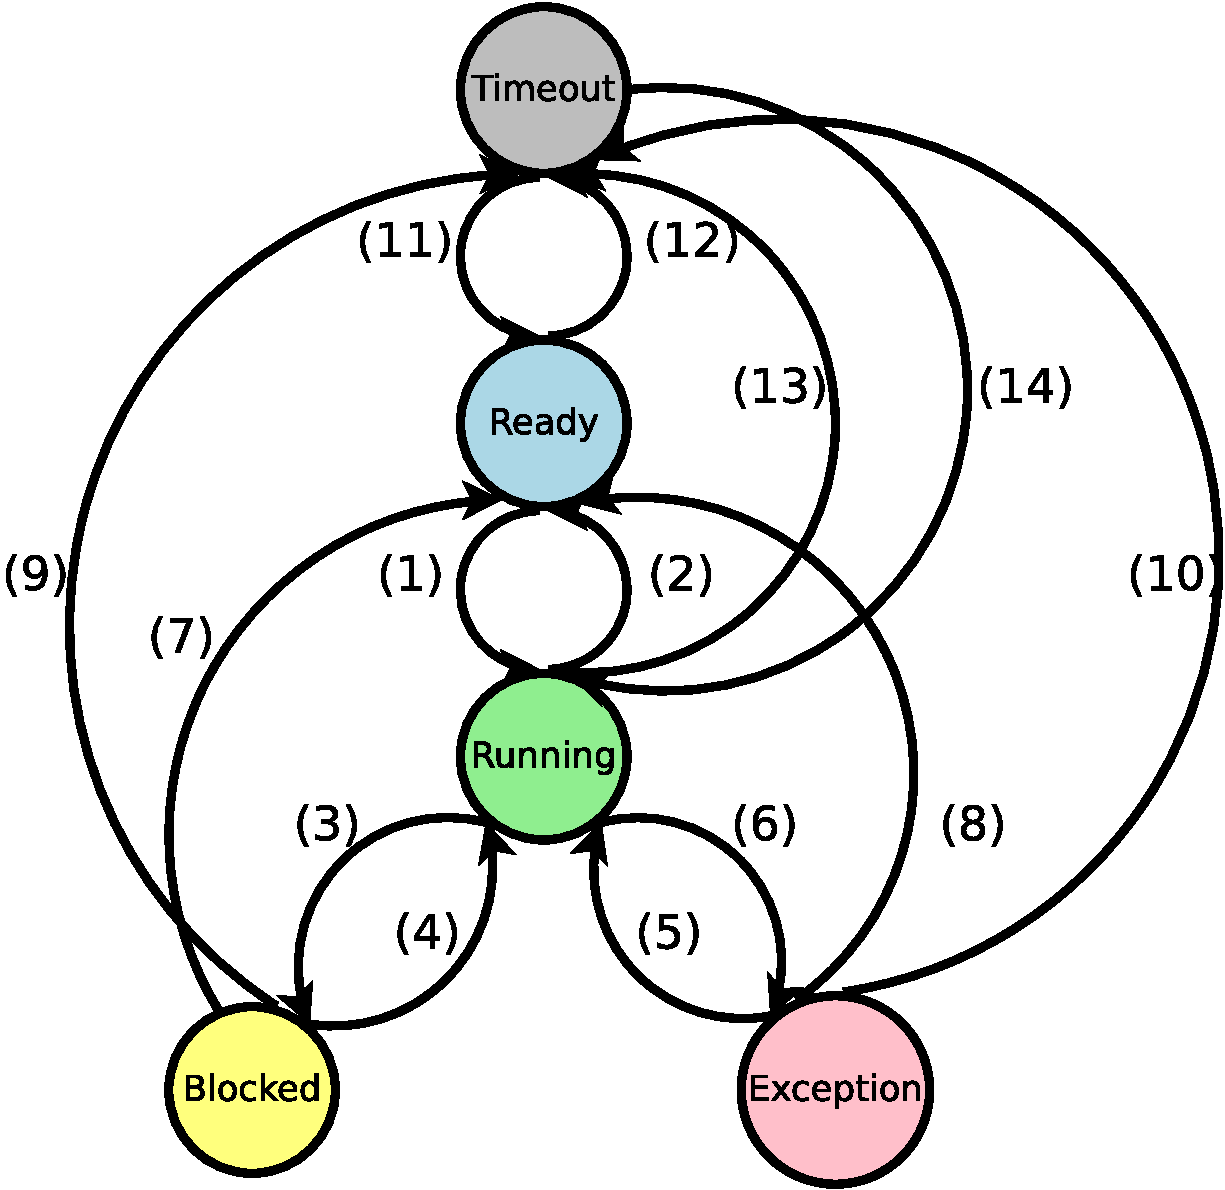
\includegraphics[width=0.72\textwidth]{Figure/image11.pdf}
    \caption{Thread State Transition Diagram}
    \label{fig:4-1-thread-state-transition-diagram}
\end{figure}

\needspace{16\baselineskip}
\newpage
The meanings of the various numeric labels in the figure are as follows:

\begin{xltabular}{\textwidth}{@{}>{\hsize=0.5279\hsize\raggedright\arraybackslash}X>{\hsize=1.4721\hsize\raggedright\arraybackslash}X@{}}
\caption{Meaning of the Labels in the Thread State Transition Diagram}\label{tab:4-7-thread-state-transition-labels}\\
\toprule
Label & Meaning\tabularnewline
\endfirsthead
\toprule
Label & Meaning\tabularnewline
\midrule
\endhead
\bottomrule
\endlastfoot
    (1) & It is the highest-priority thread on the current core, so it transitions from the ready state to the running state.\tabularnewline
    (2) & A higher-priority thread on the current core interrupted its execution, so it transitions from the running state to the ready state.\tabularnewline
    (3) & The thread blocks at a signal endpoint, so it transitions from the running state to the blocked state.\tabularnewline
    (4) & The thread received a signal from the signal endpoint, was unblocked, and is the highest-priority thread on the current core, and its timeslice has not been exhausted, so it transitions from the blocked state to the running state.\tabularnewline
    (5) & After an error occurred, the thread was restored to a normally executable state by re-setting its execution information, and it is the highest-priority thread on the current core, and its timeslice has not been exhausted, so it transitions from the exception state to the running state.\tabularnewline
    (6) & An exception occurred during the execution of the thread, so it transitions from the running state to the exception state.\tabularnewline
    (7) & The thread received a signal from the signal endpoint, was unblocked, and its timeslice has not been exhausted, but it is not the highest-priority thread on the current core, so it transitions from the blocked state to the ready state.\tabularnewline
    (8) & After an error occurred, the thread was restored to a normally executable state by re-setting its execution information, and its timeslice has not been exhausted, but it is not the highest-priority thread on the current core, so it transitions from the exception state to the ready state.\tabularnewline
    (9) & While waiting at the signal endpoint, the thread had its own timeslices transferred out by other threads, zeroing its own timeslices; therefore, after receiving a signal and being unblocked, it transitions from the blocked state to the timeout state.\tabularnewline
    (10) & After an error occurred, the thread had its own timeslices transferred out by other threads, zeroing its own timeslices; therefore, after being restored to a normally executable state by re-setting its execution information, it transitions from the exception state to the timeout state.\tabularnewline
    (11) & The thread was transferred timeslices by other threads and re-entered a state in which it can run, but it is not the highest-priority thread on the current core, so it transitions from the timeout state to the ready state.\tabularnewline
    (12) & While in the ready state, the thread had its own timeslices transferred out by other threads, zeroing its own timeslices, so it transitions from the ready state to the timeout state.\tabularnewline
    (13) & The thread exhausted its own timeslices during execution, so it transitions from the running state to the timeout state.\tabularnewline
    (14) & The thread was transferred timeslices by other threads and re-entered a state in which it can run, and it is the highest-priority thread on the current core, so it transitions from the timeout state to the running state.\tabularnewline
\end{xltabular}
\nopagebreak[4]

Among them, all transitions into the timeout state and the exception state, such as (6), (9), (10), (12) and (13), will cause a scheduler event to be sent.

\section{Process Function List}\label{sec:4-process-function-list}

The kernel functions related to processes are as follows:

\begin{xltabular}{\textwidth}{@{}>{\hsize=0.9445\hsize\raggedright\arraybackslash}X>{\hsize=0.7197\hsize\raggedright\arraybackslash}X>{\hsize=1.3358\hsize\raggedright\arraybackslash}X@{}}
\caption{Process-Related Kernel Functions}\label{tab:4-8-process-related-kernel-functions}\\
\toprule
Call Number & Type & Purpose\tabularnewline
\endfirsthead
\toprule
Call Number & Type & Purpose\tabularnewline
\midrule
\endhead
\bottomrule
\endlastfoot
RME\_SVC\_PRC\_CRT & System call & Create a process\tabularnewline
RME\_SVC\_PRC\_DEL & System call & Delete a process\tabularnewline
RME\_SVC\_PRC\_CPT & System call & Replace the capability table of a process\tabularnewline
RME\_SVC\_PRC\_PGT & System call &
Replace the page table\footnote{Top-level page directory} of a process\tabularnewline
\end{xltabular}
\nopagebreak[4]

The operation flags of a process capability are as follows:

\begin{xltabular}{\textwidth}{@{}>{\hsize=0.9158\hsize\raggedright\arraybackslash}X>{\hsize=0.6763\hsize\raggedright\arraybackslash}X>{\hsize=1.4079\hsize\raggedright\arraybackslash}X@{}}
\caption{Process Operation Flags}\label{tab:4-9-process-operation-flags}\\
\toprule
Flag & Bit & Purpose\tabularnewline
\endfirsthead
\toprule
Flag & Bit & Purpose\tabularnewline
\midrule
\endhead
\bottomrule
\endlastfoot
RME\_PRC\_FLAG\_INV & {[}0{]} &
Allows the creation of synchronous invocations within this process.\tabularnewline
RME\_PRC\_FLAG\_THD & {[}1{]} & Allows the creation of threads within this process.\tabularnewline
RME\_PRC\_FLAG\_CPT & {[}2{]} & Allows replacing the capability table of this process.\tabularnewline
RME\_PRC\_FLAG\_PGT & {[}3{]} &
Allows replacing the page table\footnote{Top-level page directory} of this process.\tabularnewline
\end{xltabular}
\nopagebreak[4]

Regarding bit {[}0{]} in the above table, please refer to \ref{subsec:5-create-sync-invocation}.

\subsection{Creating a Process}\label{subsec:4-create-a-process}

This operation creates a process and places its capability into an existing capability table. The newly created process references the capability table capability and the page directory capability; once a process has been created with a certain pair of capability table/page directory capabilities, this pair of capabilities cannot be removed/deleted before the process is deleted. A process capability has no separately allocated kernel object, so it can be created without a kernel memory capability.

Creating a process requires the following parameters:

\begin{xltabular}{\textwidth}{@{}>{\hsize=0.7639\hsize\raggedright\arraybackslash}X>{\hsize=0.6758\hsize\raggedright\arraybackslash}X>{\hsize=0.6758\hsize\raggedright\arraybackslash}X>{\hsize=1.8846\hsize\raggedright\arraybackslash}X@{}}
\caption{Parameters Needed for Process Creation}\label{tab:4-10-create-process-parameters}\\
\toprule
Parameter Name & Type & Domain & Description\tabularnewline
\endfirsthead
\toprule
Parameter Name & Type & Domain & Description\tabularnewline
\midrule
\endhead
\bottomrule
\endlastfoot
Svc\_Num & ptr\_t & N & Must be RME\_SVC\_PRC\_CRT.\tabularnewline
Cap\_Cpt\_Crt & cid\_t & C &
A capability number corresponding to a capability table capability that must have the RME\_CPT\_FLAG\_CRT attribute; the capability corresponding to this capability number points to the capability table that is to receive this newly created process capability. This capability number can be a one-level or two-level lookup encoding.\tabularnewline
Cap\_Prc & cid\_t & P0 &
A capability number corresponding to a position in the capability table that is to receive this newly created process capability. The capability corresponding to this capability number must be empty. This capability number can only be a one-level lookup encoding.\tabularnewline
Cap\_Cpt & cid\_t & P1 &
A capability number corresponding to a capability table capability that must have the RME\_CPT\_FLAG\_PRC\_CRT attribute; the capability corresponding to this capability number points to the capability table to be used by the newly created process. This capability number can be a one-level or two-level lookup encoding.\tabularnewline
Cap\_Pgt & cid\_t & P2 &
A capability number corresponding to a page table capability that must have the RME\_PGT\_FLAG\_PRC\_CRT attribute; the capability corresponding to this capability number points to the page table\footnote{Top-level page directory} to be used by the newly created process. This capability number can be a one-level or two-level lookup encoding.\tabularnewline
Raw\_Pgt & ptr\_t & P2 &
Once the user-mode page table control macro RME\_PGT\_RAW\_USER is enabled at porting time, this parameter replaces Cap\_Pgt. It is the physical address where the page table data structure directly recognizable by the processor resides, and the kernel will use it directly. Therefore, when user-mode page tables are used, user-mode processes with the process creation permission must be trusted.\tabularnewline
\end{xltabular}
\nopagebreak[4]

\needspace{16\baselineskip}
The return values of this operation may be as follows:

\begin{xltabular}{\textwidth}{@{}>{\hsize=0.8317\hsize\raggedright\arraybackslash}X>{\hsize=1.1683\hsize\raggedright\arraybackslash}X@{}}
\caption{Possible Return Values for Process Creation}\label{tab:4-11-create-process-return-values}\\
\toprule
Return Value & Meaning\tabularnewline
\endfirsthead
\toprule
Return Value & Meaning\tabularnewline
\midrule
\endhead
\bottomrule
\endlastfoot
    0 & The operation succeeded.\tabularnewline
    RME\_ERR\_CPT\_RANGE & The one-level/two-level lookup of Cap\_Cpt\_Crt is out of range.\tabularnewline
    RME\_ERR\_CPT\_RANGE & The one-level/two-level lookup of Cap\_Cpt is out of range.\tabularnewline
    RME\_ERR\_CPT\_RANGE & The one-level/two-level lookup of Cap\_Pgt is out of range.\tabularnewline
    RME\_ERR\_CPT\_RANGE & The one-level lookup of Cap\_Prc is out of range.\tabularnewline
    RME\_ERR\_CPT\_FROZEN & The capability of the one-level/two-level lookup of Cap\_Cpt\_Crt has been frozen.\tabularnewline
    RME\_ERR\_CPT\_FROZEN & The one-level/two-level lookup capability of Cap\_Cpt has been frozen.\tabularnewline
    RME\_ERR\_CPT\_FROZEN & The one-level/two-level lookup capability of Cap\_Pgt has been frozen.\tabularnewline
    RME\_ERR\_CPT\_FROZEN & Cap\_Prc has been frozen, or another core is creating a capability there.\tabularnewline
    RME\_ERR\_CPT\_TYPE & Cap\_Cpt\_Crt or Cap\_Cpt is not a capability table capability.\tabularnewline
    RME\_ERR\_CPT\_TYPE & Cap\_Pgt is not a page table capability.\tabularnewline
    RME\_ERR\_CPT\_FLAG & Cap\_Cpt\_Crt has no RME\_CPT\_FLAG\_CRT attribute.\tabularnewline
    RME\_ERR\_CPT\_FLAG & Cap\_Cpt has no RME\_CPT\_FLAG\_PRC\_CRT attribute.\tabularnewline
    RME\_ERR\_CPT\_FLAG & Cap\_Pgt has no RME\_PGT\_FLAG\_PRC\_CRT attribute.\tabularnewline
    RME\_ERR\_CPT\_EXIST & Cap\_Prc is not an empty capability.\tabularnewline
\end{xltabular}
\nopagebreak[4]

\subsection{Deleting a Process}\label{subsec:4-delete-a-process}

This operation deletes a process. The process being deleted must not contain threads or synchronous invocation calls (for the latter, see the synchronous communication mechanism). Deleting a process requires the following parameters:

\begin{xltabular}{\textwidth}{@{}>{\hsize=0.6910\hsize\raggedright\arraybackslash}X>{\hsize=0.6910\hsize\raggedright\arraybackslash}X>{\hsize=0.6910\hsize\raggedright\arraybackslash}X>{\hsize=1.9271\hsize\raggedright\arraybackslash}X@{}}
\caption{Parameters Needed for Process Deletion}\label{tab:4-12-delete-process-parameters}\\
\toprule
Parameter Name & Type & Domain & Description\tabularnewline
\endfirsthead
\toprule
Parameter Name & Type & Domain & Description\tabularnewline
\midrule
\endhead
\bottomrule
\endlastfoot
Svc\_Num & ptr\_t & N & Must be RME\_SVC\_PRC\_DEL.\tabularnewline
Cap\_Cpt & cid\_t & C &
A capability number corresponding to a capability table capability that must have the RME\_CPT\_FLAG\_DEL attribute; the capability corresponding to this capability number points to the capability table containing the process capability being deleted. This capability number can be a one-level or two-level lookup encoding.\tabularnewline
Cap\_Prc & cid\_t & P1 &
A capability number corresponding to the process capability to be deleted. The capability corresponding to this capability number must be a process capability. This capability number can only be a one-level lookup encoding.\tabularnewline
\end{xltabular}
\nopagebreak[4]

The return values of this operation may be as follows:

\begin{xltabular}{\textwidth}{@{}>{\hsize=0.6993\hsize\raggedright\arraybackslash}X>{\hsize=1.3007\hsize\raggedright\arraybackslash}X@{}}
\caption{Possible Return Values for Process Deletion}\label{tab:4-13-delete-process-return-values}\\
\toprule
Return Value & Meaning\tabularnewline
\endfirsthead
\toprule
Return Value & Meaning\tabularnewline
\midrule
\endhead
\bottomrule
\endlastfoot
    0 & The operation succeeded.\tabularnewline
    RME\_ERR\_CPT\_RANGE & The one-level/two-level lookup of Cap\_Cpt is out of range.\tabularnewline
    RME\_ERR\_CPT\_RANGE & The one-level lookup of Cap\_Prc is out of range.\tabularnewline
    RME\_ERR\_CPT\_FROZEN & The capability of the one-level/two-level lookup of Cap\_Cpt has been frozen.\tabularnewline
    RME\_ERR\_CPT\_FROZEN & Cap\_Prc has not been frozen.\tabularnewline
    RME\_ERR\_CPT\_TYPE & Cap\_Cpt is not a capability table capability.\tabularnewline
    RME\_ERR\_CPT\_TYPE & Cap\_Prc is not a process capability.\tabularnewline
    RME\_ERR\_CPT\_NULL & Cap\_Prc is an empty capability.\tabularnewline
    RME\_ERR\_CPT\_NULL & Two cores attempt to delete this process at the same time; in this case, the core that did not succeed returns this value.\tabularnewline
    RME\_ERR\_CPT\_FLAG & Cap\_Cpt has no RME\_CPT\_FLAG\_DEL attribute.\tabularnewline
    RME\_ERR\_CPT\_QUIE & Cap\_Prc is not quiescent.\tabularnewline
    RME\_ERR\_CPT\_REFCNT & The reference count of Cap\_Prc is not 0, or it is not a root capability\footnote{It internally has threads or synchronous invocation calls}.\tabularnewline
\end{xltabular}
\nopagebreak[4]

\needspace{30\baselineskip}
\subsection{Changing the Capability Table of a Process}\label{subsec:4-change-process-capability-table}
\nopagebreak[4]

This operation replaces the capability table of a process with another one. The replacement takes effect immediately after it is completed. Replacing the capability table of a process requires the following parameters:

\begin{xltabular}{\textwidth}{@{}>{\hsize=0.6910\hsize\raggedright\arraybackslash}X>{\hsize=0.6910\hsize\raggedright\arraybackslash}X>{\hsize=0.6910\hsize\raggedright\arraybackslash}X>{\hsize=1.9271\hsize\raggedright\arraybackslash}X@{}}
\caption{Parameters Needed for Changing the Capability Table of a Process}\label{tab:4-14-change-process-capability-table-parameters}\\
\toprule
Parameter Name & Type & Domain & Description\tabularnewline
\endfirsthead
\toprule
Parameter Name & Type & Domain & Description\tabularnewline
\midrule
\endhead
\bottomrule
\endlastfoot
Svc\_Num & ptr\_t & N & Must be RME\_SVC\_PRC\_CPT.\tabularnewline
Cap\_Prc & cid\_t & P1 &
A capability number corresponding to a process capability that must have the RME\_PRC\_FLAG\_CPT attribute; the capability corresponding to this capability number points to the process whose capability table is to be changed. This capability number can be a one-level or two-level lookup encoding.\tabularnewline
Cap\_Cpt & cid\_t & P2 &
A capability number corresponding to a capability table capability that must have the RME\_CPT\_FLAG\_PRC\_CPT attribute; the capability corresponding to this capability number points to the capability table to be used for the process. This capability number can be a one-level or two-level lookup encoding.\tabularnewline
\end{xltabular}
\nopagebreak[4]

The return values of this operation may be as follows:

\begin{xltabular}{\textwidth}{@{}>{\hsize=0.7784\hsize\raggedright\arraybackslash}X>{\hsize=1.2216\hsize\raggedright\arraybackslash}X@{}}
\caption{Return Values Needed for Changing the Capability Table of a Process}\label{tab:4-15-change-process-capability-table-return-values}\\
\toprule
Return Value & Meaning\tabularnewline
\endfirsthead
\toprule
Return Value & Meaning\tabularnewline
\midrule
\endhead
\bottomrule
\endlastfoot
    0 & The operation succeeded.\tabularnewline
    RME\_ERR\_CPT\_RANGE & The one-level/two-level lookup of Cap\_Prc is out of range.\tabularnewline
    RME\_ERR\_CPT\_RANGE & The one-level lookup of Cap\_Cpt is out of range.\tabularnewline
    RME\_ERR\_CPT\_FROZEN & The capability of the one-level/two-level lookup of Cap\_Prc has been frozen.\tabularnewline
    RME\_ERR\_CPT\_FROZEN & The capability of the one-level/two-level lookup of Cap\_Cpt has been frozen.\tabularnewline
    RME\_ERR\_CPT\_TYPE & Cap\_Prc is not a process capability.\tabularnewline
    RME\_ERR\_CPT\_TYPE & Cap\_Cpt is not a capability table capability.\tabularnewline
    RME\_ERR\_CPT\_NULL & Cap\_Prc or Cap\_Cpt is an empty capability.\tabularnewline
    RME\_ERR\_CPT\_FLAG & Cap\_Prc has no RME\_PRC\_FLAG\_CPT attribute.\tabularnewline
    RME\_ERR\_CPT\_FLAG & Cap\_Cpt has no RME\_CPT\_FLAG\_PRC\_CPT attribute.\tabularnewline
    RME\_ERR\_PTH\_CONFLICT & Two cores attempt to replace the capability table at the same time; in this case, the core that did not succeed returns this value.\tabularnewline
\end{xltabular}
\nopagebreak[4]

\subsection{Changing the Page Table of a Process}\label{subsec:4-change-process-page-table}

This operation replaces the page table of a process with another one. The replacement takes effect immediately after it is completed. Replacing the page table of a process requires the following parameters:

\begin{xltabular}{\textwidth}{@{}>{\hsize=0.6910\hsize\raggedright\arraybackslash}X>{\hsize=0.6910\hsize\raggedright\arraybackslash}X>{\hsize=0.6910\hsize\raggedright\arraybackslash}X>{\hsize=1.9271\hsize\raggedright\arraybackslash}X@{}}
\caption{Parameters Needed for Changing the Page Table of a Process}\label{tab:4-16-change-process-page-table-parameters}\\
\toprule
Parameter Name & Type & Domain & Description\tabularnewline
\endfirsthead
\toprule
Parameter Name & Type & Domain & Description\tabularnewline
\midrule
\endhead
\bottomrule
\endlastfoot
Svc\_Num & ptr\_t & N & Must be RME\_SVC\_PRC\_PGT.\tabularnewline
Cap\_Prc & cid\_t & P1 &
A capability number corresponding to a process capability that must have the RME\_PRC\_FLAG\_PGT attribute; the capability corresponding to this capability number points to the process whose page table\footnote{Top-level page directory} is to be changed. This capability number can be a one-level or two-level lookup encoding.\tabularnewline
Cap\_Pgt & cid\_t & P2 &
A capability number corresponding to a page directory capability that must have the RME\_PGT\_FLAG\_PRC\_PGT attribute; the capability corresponding to this capability number points to the page table\footnote{Top-level page directory} to be used for the process. This capability number can be a one-level or two-level lookup encoding.\tabularnewline
Raw\_Pgt & ptr\_t & P2 &
Once the user-mode page table control macro RME\_PGT\_RAW\_USER is enabled at porting time, this parameter replaces Cap\_Pgt. It is the physical address where the page table data structure directly recognizable by the processor resides, and the kernel will use it directly. Therefore, when user-mode page tables are used, user-mode processes with this permission must be trusted.\tabularnewline
\end{xltabular}
\nopagebreak[4]

The return values of this operation may be as follows:

\begin{xltabular}{\textwidth}{@{}>{\hsize=0.7880\hsize\raggedright\arraybackslash}X>{\hsize=1.2120\hsize\raggedright\arraybackslash}X@{}}
\caption{Possible Return Values for Changing the Page Table of a Process}\label{tab:4-17-change-process-page-table-return-values}\\
\toprule
Return Value & Meaning\tabularnewline
\endfirsthead
\toprule
Return Value & Meaning\tabularnewline
\midrule
\endhead
\bottomrule
\endlastfoot
    0 & The operation succeeded.\tabularnewline
    RME\_ERR\_CPT\_RANGE & The one-level/two-level lookup of Cap\_Prc is out of range.\tabularnewline
    RME\_ERR\_CPT\_RANGE & The one-level lookup of Cap\_Pgt is out of range.\tabularnewline
    RME\_ERR\_CPT\_FROZEN & The capability of the one-level/two-level lookup of Cap\_Prc has been frozen.\tabularnewline
    RME\_ERR\_CPT\_FROZEN & The capability of the one-level/two-level lookup of Cap\_Pgt has been frozen.\tabularnewline
    RME\_ERR\_CPT\_TYPE & Cap\_Prc is not a process capability.\tabularnewline
    RME\_ERR\_CPT\_TYPE & Cap\_Pgt is not a page table capability.\tabularnewline
    RME\_ERR\_CPT\_NULL & Cap\_Prc or Cap\_Pgt is an empty capability.\tabularnewline
    RME\_ERR\_CPT\_FLAG & Cap\_Prc has no RME\_PRC\_FLAG\_PGT attribute.\tabularnewline
    RME\_ERR\_CPT\_FLAG & Cap\_Pgt has no RME\_PGT\_FLAG\_PRC\_PGT attribute.\tabularnewline
    RME\_ERR\_PTH\_CONFLICT & Two cores attempt to replace the page table at the same time; in this case, the core that did not succeed returns this value.\tabularnewline
\end{xltabular}
\nopagebreak[4]

\section{Thread Function List}\label{sec:4-thread-function-list}

The kernel functions related to threads are as follows:

\begin{xltabular}{\textwidth}{@{}>{\hsize=1.0550\hsize\raggedright\arraybackslash}X>{\hsize=0.6673\hsize\raggedright\arraybackslash}X>{\hsize=1.2777\hsize\raggedright\arraybackslash}X@{}}
\caption{Thread Related Kernel Functions}\label{tab:4-18-thread-related-kernel-functions}\\
\toprule
Call Number & Type & Purpose\tabularnewline
\endfirsthead
\toprule
Call Number & Type & Purpose\tabularnewline
\midrule
\endhead
\bottomrule
\endlastfoot
RME\_SVC\_THD\_CRT & System Call & Create a thread\tabularnewline
RME\_SVC\_THD\_DEL & System Call & Delete a thread\tabularnewline
RME\_SVC\_THD\_SCHED\_BIND & System Call & Bind a thread to a certain CPU\tabularnewline
RME\_SVC\_THD\_SCHED\_FREE & System Call &
Free a thread from a certain CPU\footnote{Top-level page directory}\tabularnewline
RME\_SVC\_THD\_EXEC\_SET & System Call &
Set the execution attributes of a thread\footnote{Entry and stack}\tabularnewline
RME\_SVC\_THD\_SCHED\_PRIO & System Call & Change the priority of a thread\tabularnewline
RME\_SVC\_THD\_SCHED\_RCV & System Call &
Receive the scheduler events of a thread\tabularnewline
RME\_SVC\_THD\_TIME\_XFER & System Call & Transfer a timeslice between threads\tabularnewline
RME\_SVC\_THD\_SWT & System Call & Switch to a thread of the same priority\tabularnewline
\end{xltabular}
\nopagebreak[4]

The operation flags of the thread capability are as follows:

\begin{xltabular}{\textwidth}{@{}>{\hsize=1.2600\hsize\raggedright\arraybackslash}X>{\hsize=0.5400\hsize\raggedright\arraybackslash}X>{\hsize=1.2000\hsize\raggedright\arraybackslash}X@{}}
\caption{Thread Operation Flags}\label{tab:4-19-thread-operation-flags}\\
\toprule
Flag & Bit & Purpose\tabularnewline
\endfirsthead
\toprule
Flag & Bit & Purpose\tabularnewline
\midrule
\endhead
\bottomrule
\endlastfoot
RME\_THD\_FLAG\_EXEC\_SET & {[}0{]} &
Allow setting the execution attributes of this thread.\tabularnewline
RME\_THD\_FLAG\_SCHED\_CHILD & {[}1{]} &
Allow this thread to act as a child thread in a bind operation.\tabularnewline
RME\_THD\_FLAG\_SCHED\_PARENT & {[}2{]} &
Allow this thread to act as a parent thread in a bind operation.\tabularnewline
RME\_THD\_FLAG\_SCHED\_PRIO & {[}3{]} &
Allow changing the priority of this thread.\tabularnewline
RME\_THD\_FLAG\_SCHED\_FREE & {[}4{]} &
Allow removing the binding of this thread to a certain CPU.\tabularnewline
RME\_THD\_FLAG\_SCHED\_RCV & {[}5{]} &
Allow receiving the scheduler events of this thread.\tabularnewline
RME\_THD\_FLAG\_XFER\_SRC & {[}6{]} &
Allow this thread to act as the source in time transfer.\tabularnewline
RME\_THD\_FLAG\_XFER\_DST & {[}7{]} &
Allow this thread to act as the destination in time transfer.\tabularnewline
RME\_THD\_FLAG\_SWT & {[}8{]} &
Allow a switch operation to switch to this thread.\tabularnewline
\end{xltabular}
\nopagebreak[4]

\subsection{Creating a Thread}\label{subsec:4-create-a-thread}

This operation creates a thread and places its capability into an existing capability table. A newly created thread is not bound to any CPU, has no TID, and is in the RME\_THD\_TIMEOUT state. To prevent a thread from creating a thread that exceeds its own priority ceiling and thereby breaking the isolation between subsystems, no thread can create a thread with a priority ceiling higher than its own.

The thread references the process specified at creation time; once a thread has been created within a process, this process cannot be deleted before the thread is deleted. Considering that some architectures have a large number of vector registers, this operation allows a context attribute to be specified, indicating the instruction sets that the thread is permitted to enable, so as to save kernel memory usage. This operation also allows the thread to map its register set into user mode; if mapping into user mode is specified, a virtual machine monitor running in user mode can modify its context at any time, thereby greatly facilitating the programming of virtualization-related functions. If the kernel decides at configuration time not to use the virtualization mapping function\footnote{See Section~\ref{subsec:7-general-macro-definitions} for details}, this function cannot be used. Creating a thread requires the following parameters:

\begin{xltabular}{\textwidth}{@{}>{\hsize=0.6786\hsize\raggedright\arraybackslash}X>{\hsize=0.6786\hsize\raggedright\arraybackslash}X>{\hsize=0.7502\hsize\raggedright\arraybackslash}X>{\hsize=1.8926\hsize\raggedright\arraybackslash}X@{}}
\caption{Parameters Needed for Thread Creation}\label{tab:4-20-create-thread-parameters}\\
\toprule
Parameter Name & Type & Domain & Description\tabularnewline
\endfirsthead
\toprule
Parameter Name & Type & Domain & Description\tabularnewline
\midrule
\endhead
\bottomrule
\endlastfoot
Svc\_Num & ptr\_t & N{[}5:0{]} & Must be RME\_SVC\_THD\_CRT.\tabularnewline
Cap\_Cpt & cid\_t & C &
A capability number corresponding to a capability table capability that must have the RME\_CPT\_FLAG\_CRT attribute; the capability corresponding to this capability number points to the capability table that is to receive this newly created thread capability. This capability number can be a one-level or two-level lookup encoding.\tabularnewline
Cap\_Kom & cid\_t & P1.D1 &
A kernel memory capability number whose identified kernel memory range must be able to hold the thread kernel object and must have the RME\_KOM\_FLAG\_THD attribute. This capability number can be a one-level or two-level lookup encoding.\tabularnewline
Cap\_Thd & cid\_t & P1.D0 &
A capability number corresponding to a position in the capability table that is to receive this newly created thread capability. The capability corresponding to this capability number must be empty. This capability number can only be a one-level lookup encoding.\tabularnewline
Cap\_Prc & cid\_t & P2.D1 &
A capability number corresponding to a process capability that must have the RME\_PRC\_FLAG\_THD attribute; the capability corresponding to this capability number points to the process that contains the newly created thread. This capability number can be a one-level or two-level lookup encoding.\tabularnewline
Max\_Prio & ptr\_t & P2.D0 & The priority ceiling of this thread.\tabularnewline
Raddr & ptr\_t & P3 &
The starting relative virtual address in kernel space to be used by the newly created thread kernel object. This address is relative to the starting virtual address of the kernel capability corresponding to Cap\_Kom.\tabularnewline
Attr & ptr\_t & N{[}X/2-1:7{]} &
Specify the extended instruction set context attributes of the thread. For different architectures, this parameter has different meanings, but in all architectures 0 means that no instruction set extension is performed and no coprocessor register state is allocated, saved or restored. For 32-bit processors, this parameter has 9 bits; for 64-bit processors, this parameter has 25 bits.\tabularnewline
Is\_Hyp & ptr\_t & N{[}6{]} &
If set to 0, the system allocates space in the kernel to save the thread context, which is the normal case. If it is not 0, the thread will map its registers into user mode, in which case the specific mapping address needs to be set when binding the thread to a CPU.\tabularnewline
\end{xltabular}
\nopagebreak[4]

The return values of this operation may be as follows:

\begin{xltabular}{\textwidth}{@{}>{\hsize=0.6791\hsize\raggedright\arraybackslash}X>{\hsize=1.3209\hsize\raggedright\arraybackslash}X@{}}
\caption{Possible Return Values for Thread Creation}\label{tab:4-21-create-thread-return-values}\\
\toprule
Return Value & Meaning\tabularnewline
\endfirsthead
\toprule
Return Value & Meaning\tabularnewline
\midrule
\endhead
\bottomrule
\endlastfoot
    0 & The operation succeeded.\tabularnewline
    RME\_ERR\_CPT\_RANGE & The one-level/two-level lookup of Cap\_Cpt is out of range.\tabularnewline
    RME\_ERR\_CPT\_RANGE & The one-level/two-level lookup of Cap\_Kom is out of range.\tabularnewline
    RME\_ERR\_CPT\_RANGE & The one-level/two-level lookup of Cap\_Prc is out of range.\tabularnewline
    RME\_ERR\_CPT\_RANGE & The one-level lookup of Cap\_Thd is out of range.\tabularnewline
    RME\_ERR\_CPT\_FROZEN & The capability of the one-level/two-level lookup of Cap\_Cpt has been frozen.\tabularnewline
    RME\_ERR\_CPT\_FROZEN & The capability of the one-level/two-level lookup of Cap\_Kom has been frozen.\tabularnewline
    RME\_ERR\_CPT\_FROZEN & The one-level/two-level lookup capability of Cap\_Prc has been frozen.\tabularnewline
    RME\_ERR\_CPT\_FROZEN & Cap\_Thd has been frozen, or another core is creating a capability there.\tabularnewline
    RME\_ERR\_CPT\_TYPE & Cap\_Cpt is not a capability table capability.\tabularnewline
    RME\_ERR\_CPT\_TYPE & Cap\_Kom is not a kernel memory capability.\tabularnewline
    RME\_ERR\_CPT\_TYPE & Cap\_Prc is not a process capability.\tabularnewline
    RME\_ERR\_CPT\_FLAG & Cap\_Cpt has no RME\_CPT\_FLAG\_CRT attribute.\tabularnewline
    RME\_ERR\_CPT\_FLAG & Cap\_Kom has no RME\_KOM\_FLAG\_THD attribute, or the range is incorrect.\tabularnewline
    RME\_ERR\_CPT\_FLAG & Cap\_Prc has no RME\_PRC\_FLAG\_THD attribute.\tabularnewline
    RME\_ERR\_CPT\_EXIST & Cap\_Thd is not an empty capability.\tabularnewline
    RME\_ERR\_CPT\_KOT & Allocation of kernel memory failed.\tabularnewline
    RME\_ERR\_PTH\_PRIO & Attempting to create a thread with a higher priority ceiling than its own, or the passed priority ceiling is too large and exceeds the limit allowed by the system configuration.\tabularnewline
\bottomrule
\end{xltabular}
\nopagebreak[4]

\needspace{30\baselineskip}
\subsection{Deleting a Thread}\label{subsec:4-delete-a-thread}
\nopagebreak[4]

This operation deletes a thread. The thread being deleted must already have been unbound. Deleting a thread requires the following parameters:

\begin{xltabular}{\textwidth}{@{}>{\hsize=0.6910\hsize\raggedright\arraybackslash}X>{\hsize=0.6910\hsize\raggedright\arraybackslash}X>{\hsize=0.6910\hsize\raggedright\arraybackslash}X>{\hsize=1.9271\hsize\raggedright\arraybackslash}X@{}}
\caption{Parameters Needed for Thread Deletion}\label{tab:4-22-delete-thread-parameters}\\
\toprule
Parameter Name & Type & Domain & Description\tabularnewline
\endfirsthead
\toprule
Parameter Name & Type & Domain & Description\tabularnewline
\midrule
\endhead
Svc\_Num & ptr\_t & N & Must be RME\_SVC\_THD\_DEL.\tabularnewline
Cap\_Cpt & cid\_t & C &
A capability number corresponding to a capability table capability that must have the RME\_CPT\_FLAG\_DEL attribute; the capability corresponding to this capability number points to the capability table containing the thread capability being deleted. This capability number can be a one-level or two-level lookup encoding.\tabularnewline
Cap\_Thd & cid\_t & P1 &
A capability number corresponding to the thread capability to be deleted. The capability corresponding to this capability number must be a thread capability. This capability number can only be a one-level lookup encoding.\tabularnewline
\end{xltabular}
\nopagebreak[4]

The return values of this operation may be as follows:

\begin{xltabular}{\textwidth}{@{}>{\hsize=0.7784\hsize\raggedright\arraybackslash}X>{\hsize=1.2216\hsize\raggedright\arraybackslash}X@{}}
\caption{Possible Return Values for Thread Deletion}\label{tab:4-23-delete-thread-return-values}\\
\toprule
Return Value & Meaning\tabularnewline
\endfirsthead
\toprule
Return Value & Meaning\tabularnewline
\midrule
\endhead
\bottomrule
\endlastfoot
    0 & The operation succeeded.\tabularnewline
    RME\_ERR\_CPT\_RANGE & The one-level/two-level lookup of Cap\_Cpt is out of range.\tabularnewline
    RME\_ERR\_CPT\_RANGE & The one-level lookup of Cap\_Thd is out of range.\tabularnewline
    RME\_ERR\_CPT\_FROZEN & The capability of the one-level/two-level lookup of Cap\_Cpt has been frozen.\tabularnewline
    RME\_ERR\_CPT\_FROZEN & Cap\_Thd has not been frozen.\tabularnewline
    RME\_ERR\_CPT\_TYPE & Cap\_Cpt is not a capability table capability.\tabularnewline
    RME\_ERR\_CPT\_TYPE & Cap\_Thd is not a thread capability.\tabularnewline
    RME\_ERR\_CPT\_NULL & Cap\_Thd is an empty capability.\tabularnewline
    RME\_ERR\_CPT\_NULL & Two cores attempt to delete this thread at the same time; in this case, the core that did not succeed returns this value.\tabularnewline
    RME\_ERR\_CPT\_FLAG & Cap\_Cpt has no RME\_CPT\_FLAG\_DEL attribute.\tabularnewline
    RME\_ERR\_CPT\_QUIE & Cap\_Thd is not quiescent.\tabularnewline
    RME\_ERR\_CPT\_REFCNT & The reference count of Cap\_Thd is not 0, or it is not a root capability.\tabularnewline
    RME\_ERR\_PTH\_INVSTATE & The thread is still in the bound state.\tabularnewline
\end{xltabular}
\nopagebreak[4]

\subsection{Binding a Thread to a CPU}\label{subsec:4-bind-a-thread-to-a-cpu}

This operation binds a thread to a certain CPU. The thread being set must not be bound to any CPU. The binding is completed on the CPU on which this function is called. For those threads that wish to map their register context into user mode for convenient modification, this operation also sets the mapping address of the context: the management of this address range is entirely the responsibility of a trusted daemon in user mode, and at boot time the kernel only guarantees that this address can be accessed both from kernel mode and from user mode, and that it will not cause a page fault. Binding a thread to a CPU requires the following parameters:

\begin{xltabular}{\textwidth}{@{}>{\hsize=0.8146\hsize\raggedright\arraybackslash}X>{\hsize=0.6652\hsize\raggedright\arraybackslash}X>{\hsize=0.6652\hsize\raggedright\arraybackslash}X>{\hsize=1.8550\hsize\raggedright\arraybackslash}X@{}}
\caption{Parameters Needed for Binding a Thread to a CPU}\label{tab:4-24-bind-thread-to-cpu-parameters}\\
\toprule
Parameter Name & Type & Domain & Description\tabularnewline
\endfirsthead
\toprule
Parameter Name & Type & Domain & Description\tabularnewline
\midrule
\endhead
\bottomrule
\endlastfoot
Svc\_Num & ptr\_t & N & Must be RME\_SVC\_THD\_SCHED\_BIND.\tabularnewline
Cap\_Thd & cid\_t & C &
A capability number corresponding to a thread capability that must have the RME\_THD\_FLAG\_SCHED\_CHILD attribute; the capability corresponding to this capability number points to the thread being bound. This capability number can be a one-level or two-level lookup encoding.\tabularnewline
Cap\_Thd\_Sched & cid\_t & P1.D1 &
A capability number corresponding to a thread capability that must have the RME\_THD\_FLAG\_SCHED\_PARENT attribute; the capability corresponding to this capability number points to the parent thread of the thread being bound. This parent thread must already be bound to the CPU on which this function is called. This capability number can be a one-level or two-level lookup encoding.\tabularnewline
Cap\_Sig & cid\_t & P1.D0 &
A capability number corresponding to a signal endpoint capability that must have the RME\_SIG\_FLAG\_SCHED attribute. When a scheduler event occurs\footnote{A thread timeout or error, where a timeout may be caused by the thread consuming all of its timeslice while running or by its timeslice being completely transferred to other threads}, this endpoint will receive a signal. This capability number can be a one-level or two-level lookup encoding, and is also optional. If scheduler signals are not desired, RME\_CID\_NULL\footnote{A half-word-length INT\_MIN (a negative value), which is 0x8000 on 32-bit systems and 0x80000000 on 64-bit systems} can be passed in.\tabularnewline
TID & tid\_t & P2.D1 &
A user-provided TID. RME itself does not check whether two threads in the system have the same ID; whether to perform such a check is a matter for user mode.\tabularnewline
Prio & ptr\_t & P2.D0 &
The preemption priority of the thread being bound. In RME, thread priorities are counted from 0, and the larger the value, the higher the priority. This value cannot exceed the inherent priority ceiling of the thread.\tabularnewline
Haddr & ptr\_t & P3 &
The mapping address of the user-mode register context. This address must lie within the address range dedicated in the system to thread context mapping, that is, greater than or equal to the base address RME\_HYP\_VA\_BASE and less than the end address RME\_HYP\_VA\_BASE+
RME\_HYP\_SIZE, and it must be aligned to a word. For ordinary threads, setting it to NULL is sufficient.\tabularnewline
\end{xltabular}
\nopagebreak[4]

The return values of this operation may be as follows:

\begin{xltabular}{\textwidth}{@{}>{\hsize=0.7880\hsize\raggedright\arraybackslash}X>{\hsize=1.2120\hsize\raggedright\arraybackslash}X@{}}
\caption{Possible Return Values for Binding a Thread to a CPU}\label{tab:4-25-bind-thread-to-cpu-return-values}\\
\toprule
Return Value & Meaning\tabularnewline
\endfirsthead
\toprule
Return Value & Meaning\tabularnewline
\midrule
\endhead
\bottomrule
\endlastfoot
    0 & The operation succeeded.\tabularnewline
    RME\_ERR\_CPT\_RANGE & The one-level/two-level lookup of Cap\_Thd or Cap\_Thd\_Sched is out of range.\tabularnewline
    RME\_ERR\_CPT\_FROZEN & The capability of the one-level/two-level lookup of Cap\_Thd or Cap\_Thd\_Sched has been frozen.\tabularnewline
    RME\_ERR\_CPT\_TYPE & Cap\_Thd or Cap\_Thd\_Sched is not a thread capability, or is an empty capability.\tabularnewline
    RME\_ERR\_CPT\_FLAG & Cap\_Thd has no RME\_THD\_FLAG\_SCHED\_CHILD attribute.\tabularnewline
    RME\_ERR\_CPT\_FLAG & Cap\_Thd\_Sched has no RME\_THD\_FLAG\_SCHED\_PARENT attribute.\tabularnewline
    RME\_ERR\_CPT\_FLAG & When Cap\_Sig is passed in, it has no RME\_SIG\_FLAG\_SCHED attribute.\tabularnewline
    RME\_ERR\_CPT\_FLAG & The processor to be bound to does not support the Attr registered when this thread was created.\tabularnewline
    RME\_ERR\_PTH\_HADDR & The Haddr passed in is not within the range allowed by the system and is invalid.\tabularnewline
    RME\_ERR\_PTH\_NOTIF & An attempt was made to register itself as its own parent thread, which is invalid.\tabularnewline
    RME\_ERR\_PTH\_PRIO & The preemption priority exceeds the inherent priority ceiling of this thread, which is invalid.\tabularnewline
    RME\_ERR\_PTH\_INVSTATE & Cap\_Thd is in the bound state or Cap\_Thd\_Sched is in the unbound state.\tabularnewline
    RME\_ERR\_PTH\_INVSTATE & Cap\_Thd\_Sched is bound to a CPU different from the CPU calling this function.\tabularnewline
    RME\_ERR\_PTH\_CONFLICT & If two CPUs attempt to bind at the same time, this value is returned on the CPU that failed.\tabularnewline
\end{xltabular}
\nopagebreak[4]

\subsection{Unbinding a Thread from a CPU}\label{subsec:4-unbind-a-thread-from-a-cpu}

This operation unbinds a thread from a CPU. The thread being unbound must not itself have child threads. If the thread being unbound has sent a scheduler event to its parent thread, then this event is revoked. If the thread being unbound blocks, then it simultaneously causes this blocking receive to be forcibly terminated and returns RME\_ERR\_SIV\_FREE. Unbinding a thread from a CPU requires the following parameters:

\begin{xltabular}{\textwidth}{@{}>{\hsize=0.6910\hsize\raggedright\arraybackslash}X>{\hsize=0.6910\hsize\raggedright\arraybackslash}X>{\hsize=0.6910\hsize\raggedright\arraybackslash}X>{\hsize=1.9271\hsize\raggedright\arraybackslash}X@{}}
\caption{Parameters Needed for Unbinding a Thread from a CPU}\label{tab:4-26-unbind-thread-from-cpu-parameters}\\
\toprule
Parameter Name & Type & Domain & Description\tabularnewline
\endfirsthead
\toprule
Parameter Name & Type & Domain & Description\tabularnewline
\midrule
\endhead
\bottomrule
\endlastfoot
Svc\_Num & ptr\_t & N &
Must be RME\_SVC\_THD\_SCHED\_FREE.\tabularnewline
Cap\_Thd & cid\_t & P1 &
A capability number corresponding to a thread capability that must have the RME\_THD\_FLAG\_SCHED\_FREE attribute; the capability corresponding to this capability number points to the thread to be unbound. This capability number can be a one-level or two-level lookup encoding.\tabularnewline
\end{xltabular}
\nopagebreak[4]

The return values of this operation may be as follows:

\begin{xltabular}{\textwidth}{@{}>{\hsize=0.7905\hsize\raggedright\arraybackslash}X>{\hsize=1.2095\hsize\raggedright\arraybackslash}X@{}}
\caption{Possible Return Values for Unbinding a Thread from a CPU}\label{tab:4-27-unbind-thread-from-cpu-return-values}\\
\toprule
Return Value & Meaning\tabularnewline
\endfirsthead
\toprule
Return Value & Meaning\tabularnewline
\midrule
\endhead
\bottomrule
\endlastfoot
    0 & The operation succeeded.\tabularnewline
    RME\_ERR\_CPT\_RANGE & The one-level/two-level lookup of Cap\_Thd is out of range.\tabularnewline
    RME\_ERR\_CPT\_FROZEN & The capability of the one-level/two-level lookup of Cap\_Thd has been frozen.\tabularnewline
    RME\_ERR\_CPT\_TYPE & Cap\_Thd is not a thread capability, or is an empty capability.\tabularnewline
    RME\_ERR\_CPT\_FLAG & Cap\_Thd has no RME\_THD\_FLAG\_SCHED\_FREE attribute.\tabularnewline
    RME\_ERR\_PTH\_REFCNT & Cap\_Thd is still the parent thread of some threads\footnote{scheduler threads}.\tabularnewline
    RME\_ERR\_PTH\_INVSTATE & Cap\_Thd is in the unbound state.\tabularnewline
    RME\_ERR\_PTH\_INVSTATE & Cap\_Thd is bound to a CPU different from the CPU calling this function.\tabularnewline
\end{xltabular}
\nopagebreak[4]

\newpage
\subsection{Setting Thread Execution Attributes}\label{subsec:4-set-thread-execution-attributes}

This operation sets the execution attributes of a thread, that is, its entry, stack, and parameters. The thread being configured must already be bound to a CPU, and setting the execution attributes must be performed on this CPU. For a thread that is already in the RME\_THD\_EXCPEND state, setting the thread execution attributes sets it to the RME\_THD\_READY or RME\_THD\_TIMEOUT state depending on its current number of timeslices, where the latter sends a scheduler event. When both the Entry and Stack passed in are NULL, the execution attributes of this thread remain unchanged and only its state is changed, which is very useful in exception handling. Setting thread execution attributes requires the following parameters:

\begin{xltabular}{\textwidth}{@{}>{\hsize=0.6910\hsize\raggedright\arraybackslash}X>{\hsize=0.6910\hsize\raggedright\arraybackslash}X>{\hsize=0.6910\hsize\raggedright\arraybackslash}X>{\hsize=1.9271\hsize\raggedright\arraybackslash}X@{}}
\caption{Parameters Needed for Setting Thread Execution Attributes}\label{tab:4-28-set-thread-execution-attributes-parameters}\\
\toprule
Parameter Name & Type & Domain & Description\tabularnewline
\endfirsthead
\toprule
Parameter Name & Type & Domain & Description\tabularnewline
\midrule
\endhead
\bottomrule
\endlastfoot
Svc\_Num & ptr\_t & N & Must be RME\_SVC\_THD\_EXEC\_SET.\tabularnewline
Cap\_Thd & cid\_t & C &
A capability number corresponding to a thread capability that must have the RME\_THD\_FLAG\_EXEC\_SET attribute; the capability corresponding to this capability number points to the thread whose execution attributes are being set. This capability number can be a one-level or two-level lookup encoding.\tabularnewline
Entry & ptr\_t & P1 &
The entry of this thread. This value is a virtual address inside the process in which the thread resides, and the thread will start executing from here. If NULL is passed in, no actual change is made.\tabularnewline
Stack & ptr\_t & P2 &
The execution stack of this thread. This value is a virtual address inside the process in which the thread resides, and the thread will use this address as the start of the stack. Whether the specific stack is an ascending stack or a descending stack is determined by the user-mode library. If NULL is passed in, no actual change is made.\tabularnewline
Param & ptr\_t & P3 & The parameter to be passed to this thread.\tabularnewline
\end{xltabular}
\nopagebreak[4]

The return values of this operation may be as follows:

\begin{xltabular}{\textwidth}{@{}>{\hsize=0.8314\hsize\raggedright\arraybackslash}X>{\hsize=1.1686\hsize\raggedright\arraybackslash}X@{}}
\caption{Possible Return Values for Setting Thread Execution Attributes}\label{tab:4-29-set-thread-execution-attributes-return-values}\\
\toprule
Return Value & Meaning\tabularnewline
\endfirsthead
\toprule
Return Value & Meaning\tabularnewline
\midrule
\endhead
\bottomrule
\endlastfoot
    0 & The operation succeeded.\tabularnewline
    RME\_ERR\_CPT\_RANGE & The one-level/two-level lookup of Cap\_Thd is out of range.\tabularnewline
    RME\_ERR\_CPT\_FROZEN & The capability of the one-level/two-level lookup of Cap\_Thd has been frozen.\tabularnewline
    RME\_ERR\_CPT\_TYPE & Cap\_Thd is not a thread capability, or is an empty capability.\tabularnewline
    RME\_ERR\_CPT\_FLAG & Cap\_Thd has no RME\_THD\_FLAG\_EXEC\_SET attribute.\tabularnewline
    RME\_ERR\_PTH\_INVSTATE & The thread is in the unbound state.\tabularnewline
\end{xltabular}
\nopagebreak[4]

\subsection{Changing Thread Priority}\label{subsec:4-change-thread-priority}

\needspace{16\baselineskip}
This operation changes the priorities of up to four threads already bound to a CPU at one time. When more than one thread is specified, these priority change operations are transactional (Transactional): they either all succeed or all fail. When fewer than four threads are specified, the unused parameters may be left unfilled. All priority change operations must be performed on the same CPU. Changing thread priority requires the following parameters:

\begin{xltabular}{\textwidth}{@{}>{\hsize=0.6910\hsize\raggedright\arraybackslash}X>{\hsize=0.6910\hsize\raggedright\arraybackslash}X>{\hsize=0.6910\hsize\raggedright\arraybackslash}X>{\hsize=1.9271\hsize\raggedright\arraybackslash}X@{}}
\caption{Parameters Needed for Changing Thread Priority}\label{tab:4-30-change-thread-priority-parameters}\\
\toprule
Parameter Name & Type & Domain & Description\tabularnewline
\endfirsthead
\toprule
Parameter Name & Type & Domain & Description\tabularnewline
\midrule
\endhead
\bottomrule
\endlastfoot
Svc\_Num & ptr\_t & N & Must be RME\_SVC\_THD\_SCHED\_PRIO.\tabularnewline
Number & ptr\_t & C &
Specifies the number of threads whose priorities need to be modified; the allowed values are 1\textasciitilde4.\tabularnewline
Cap\_Thd0 & cid\_t & P1.D0 &
A capability number corresponding to a thread capability that must have the RME\_THD\_FLAG\_SCHED\_PRIO attribute; the capability corresponding to this capability number points to the thread whose preemption priority is to be modified. This capability number can be a one-level or two-level lookup encoding.\tabularnewline
Prio0 & ptr\_t & P3.Q0 &
The new preemption priority of the thread. In RME, thread priorities are counted from 0, and the larger the value, the higher the priority. This value cannot exceed the inherent priority ceiling of this thread.\tabularnewline
Cap\_Thd1 & cid\_t & P1.D1 & The capability number of the second thread (optional).\tabularnewline
Prio1 & ptr\_t & P3.Q1 &
The new preemption priority of the second thread (optional).\tabularnewline
Cap\_Thd2 & cid\_t & P2.D0 & The capability number of the third thread (optional).\tabularnewline
Prio2 & ptr\_t & P3.Q2 &
The new preemption priority of the third thread (optional).\tabularnewline
Cap\_Thd3 & cid\_t & P2.D1 & The capability number of the fourth thread (optional).\tabularnewline
Prio3 & ptr\_t & P3.Q3 &
The new preemption priority of the fourth thread (optional).\tabularnewline
\end{xltabular}
\nopagebreak[4]

The return values of this operation may be as follows:

\begin{xltabular}{\textwidth}{@{}>{\hsize=0.7437\hsize\raggedright\arraybackslash}X>{\hsize=1.2563\hsize\raggedright\arraybackslash}X@{}}
\caption{Possible Return Values for Changing Thread Priority}\label{tab:4-31-change-thread-priority-return-values}\\
\toprule
Return Value & Meaning\tabularnewline
\endfirsthead
\toprule
Return Value & Meaning\tabularnewline
\midrule
\endhead
\bottomrule
\endlastfoot
    0 & The operation succeeded.\tabularnewline
    RME\_ERR\_CPT\_RANGE & The one-level/two-level lookup of at least one of the four Cap\_Thd is out of range.\tabularnewline
    RME\_ERR\_CPT\_FROZEN & The capability of the one-level/two-level lookup of at least one of the four Cap\_Thd has been frozen.\tabularnewline
    RME\_ERR\_CPT\_TYPE & At least one of the four Cap\_Thd is not a thread capability, or is an empty capability.\tabularnewline
    RME\_ERR\_CPT\_FLAG & At least one of the four Cap\_Thd has no RME\_THD\_FLAG\_SCHED\_PRIO attribute.\tabularnewline
    RME\_ERR\_PTH\_PRIO & The priority of at least one thread exceeds the inherent priority ceiling of this thread, which is invalid.\tabularnewline
    RME\_ERR\_PTH\_PRIO & The value of Number is not in the range 1~4.\tabularnewline
    RME\_ERR\_PTH\_INVSTATE & At least one thread is in the unbound state.\tabularnewline
    RME\_ERR\_PTH\_INVSTATE & At least one thread is bound to a CPU different from the CPU calling this function.\tabularnewline
\end{xltabular}
\nopagebreak[4]

\needspace{30\baselineskip}
\subsection{Receiving a Thread's Scheduler Event}\label{subsec:4-receive-thread-scheduler-event}
\nopagebreak[4]

This operation receives a scheduler event of a thread. This operation does not block; if the thread has no scheduler event for the time being, then we return a negative value. If the returned value is positive, then it may consist of three parts: the exception identifier RME\_THD\_EXCPEND\_FLAG\footnote{the second-to-last binary bit}, the timeslice exhaustion identifier RME\_THD\_TIMEOUT\_FLAG\footnote{the third-to-last binary bit}, and the thread identifier TID\footnote{the other, subsequent binary bits}.

If RME\_THD\_EXCPEND\_FLAG is set, it indicates that the thread is in the exception state; at this point, the kernel function call described in \ref{subsec:8-get-thread-exception-register-set}
can be used to query the cause of the exception, and RME\_SVC\_THD\_EXEC\_SET can be used to clear the exception and continue execution; if RME\_THD\_TIMEOUT\_FLAG is set, it indicates that the thread is in the timeout state, and at this point RME\_SVC\_THD\_TIME\_XFER can be used to transfer more timeslices to it. These two identifiers may be present at the same time: when they are both present, it indicates that the thread is in the exception state and holds 0 timeslices; once its execution attributes are set to clear its exception state, the thread will immediately enter the timeout state\footnote{This transition from the exception state to the timeout state also sends a scheduler event}.

Receiving the scheduler event of a thread requires the following parameters:

\begin{xltabular}{\textwidth}{@{}>{\hsize=0.6910\hsize\raggedright\arraybackslash}X>{\hsize=0.6910\hsize\raggedright\arraybackslash}X>{\hsize=0.6910\hsize\raggedright\arraybackslash}X>{\hsize=1.9271\hsize\raggedright\arraybackslash}X@{}}
\caption{Parameters Needed for Receiving a Thread's Scheduler Event}\label{tab:4-32-receive-thread-scheduler-event-parameters}\\
\toprule
Parameter Name & Type & Domain & Description\tabularnewline
\endfirsthead
\toprule
Parameter Name & Type & Domain & Description\tabularnewline
\midrule
\endhead
\bottomrule
\endlastfoot
Svc\_Num & ptr\_t & N & Must be RME\_SVC\_THD\_SCHED\_RCV.\tabularnewline
Cap\_Thd & cid\_t & P1 &
A capability number corresponding to a thread capability that must have the RME\_THD\_FLAG\_SCHED\_RCV attribute; we attempt to receive the scheduler events sent from the child threads of this thread. This capability number can be a one-level or two-level lookup encoding.\tabularnewline
\end{xltabular}
\nopagebreak[4]

\needspace{16\baselineskip}
The return values of this operation may be as follows:

\begin{xltabular}{\textwidth}{@{}>{\hsize=0.7023\hsize\raggedright\arraybackslash}X>{\hsize=1.2977\hsize\raggedright\arraybackslash}X@{}}
\caption{Possible Return Values for Receiving a Thread's Scheduler Event}\label{tab:4-33-receive-thread-scheduler-event-return-values}\\
\toprule
Return Value & Meaning\tabularnewline
\endfirsthead
\toprule
Return Value & Meaning\tabularnewline
\midrule
\endhead
\bottomrule
\endlastfoot
    Non-negative value & The operation succeeded. If the error identifier is 0, then what was received is a thread timeout event, indicating that the thread corresponding to the thread identifier exhausted its timeslice and stopped executing. If the error identifier is 1, then it indicates that the thread corresponding to the thread identifier encountered an error during execution and was forced to stop executing.\tabularnewline
    RME\_ERR\_CPT\_RANGE & The one-level/two-level lookup of Cap\_Thd is out of range.\tabularnewline
    RME\_ERR\_CPT\_FROZEN & The capability of the one-level/two-level lookup of Cap\_Thd has been frozen.\tabularnewline
    RME\_ERR\_CPT\_TYPE & Cap\_Thd is not a thread capability, or is an empty capability.\tabularnewline
    RME\_ERR\_CPT\_FLAG & Cap\_Thd has no RME\_THD\_FLAG\_SCHED\_RCV attribute.\tabularnewline
    RME\_ERR\_PTH\_NOTIF & Cap\_Thd has no scheduler event available to receive for the time being.\tabularnewline
    RME\_ERR\_PTH\_INVSTATE & Cap\_Thd is in the unbound state.\tabularnewline
    RME\_ERR\_PTH\_INVSTATE & Cap\_Thd is bound to a CPU different from the CPU calling this function.\tabularnewline
\end{xltabular}
\nopagebreak[4]

\subsection{Transferring Run Time Slice Between Threads}\label{subsec:4-transfer-run-time-slice-between-threads}

This operation is used to transfer timeslices between threads. The source thread\footnote{source thread} and the destination thread\footnote{destination thread} of the timeslice must be bound to the same CPU, and this system call must be performed on this CPU, to ensure that the transferred time is execution time on this CPU. The timeslice held by the source thread itself and the timeslice to be transferred must not be 0. If the source thread loses all of its timeslices when transferring, it immediately sends a scheduler event to its scheduler thread.

This function allows a low-priority thread to transfer run time slices to a high-priority thread, but does not allow a thread with a low priority ceiling to transfer run time slices to a thread with a high priority ceiling\footnote{Except for the Init thread; as a special case, transferring timeslices to the Init thread to void time is permitted}: this is to ensure that timeslices always degrade (Degrade) during transfer, so that low-priority subsystems do not interfere with high-priority subsystems.

Transferring run time slices requires the following parameters:

\begin{xltabular}{\textwidth}{@{}>{\hsize=0.7639\hsize\raggedright\arraybackslash}X>{\hsize=0.6758\hsize\raggedright\arraybackslash}X>{\hsize=0.6758\hsize\raggedright\arraybackslash}X>{\hsize=1.8846\hsize\raggedright\arraybackslash}X@{}}
\caption{Parameters Needed for Transferring Run Time Slice Between Threads}\label{tab:4-34-transfer-run-time-slice-between-threads-parameters}\\
\toprule
Parameter Name & Type & Domain & Description\tabularnewline
\endfirsthead
\toprule
Parameter Name & Type & Domain & Description\tabularnewline
\midrule
\endhead
\bottomrule
\endlastfoot
Svc\_Num & ptr\_t & N & Must be RME\_SVC\_THD\_TIME\_XFER.\tabularnewline
Cap\_Thd\_Dst & cid\_t & P1 &
A capability number corresponding to a thread capability that must have the RME\_THD\_FLAG\_XFER\_DST attribute; the capability corresponding to this capability number points to the destination thread. This capability number can be a one-level or two-level lookup encoding.\tabularnewline
Cap\_Thd\_Src & cid\_t & P2 &
A capability number corresponding to a thread capability that must have the RME\_THD\_FLAG\_XFER\_SRC attribute; the capability corresponding to this capability number points to the source thread. This capability number can be a one-level or two-level lookup encoding.\tabularnewline
Time\strut
 & ptr\_t\strut
 & P3\strut
 & The number of timeslices to transfer. The unit of this value is the timeslice; the size of a single timeslice is determined at system compile time. This value cannot be 0.

Pass in RME\_THD\_INF\_TIME for an infinite transfer.

Pass in RME\_THD\_INIT\_TIME for a revoking transfer.

Pass in any other non-zero value for a normal transfer.\strut
\tabularnewline
\end{xltabular}
\nopagebreak[4]

The return values of this operation may be as follows:

\begin{xltabular}{\textwidth}{@{}>{\hsize=1.0000\hsize\raggedright\arraybackslash}X>{\hsize=1.0000\hsize\raggedright\arraybackslash}X@{}}
\caption{Possible Return Values for Transferring Run Time Slice Between Threads}\label{tab:4-35-transfer-run-time-slice-between-threads-return-values}\\
\toprule
Return Value & Meaning\tabularnewline
\endfirsthead
\toprule
Return Value & Meaning\tabularnewline
\midrule
\endhead
\bottomrule
\endlastfoot
    Non-negative value & The operation succeeded, and what is returned is the current number of timeslices of the destination thread. If an infinite transfer or a revoking transfer is performed and the destination thread has become an infinite thread, then RME\_THD\_INF\_TIME is returned.\tabularnewline
    RME\_ERR\_CPT\_RANGE & The one-level/two-level lookup of Cap\_Thd\_Dst or Cap\_Thd\_Src is out of range.\tabularnewline
    RME\_ERR\_CPT\_FROZEN & The capability of the one-level/two-level lookup of Cap\_Thd\_Dst or Cap\_Thd\_Src has been frozen.\tabularnewline
    RME\_ERR\_CPT\_TYPE & Cap\_Thd\_Dst or Cap\_Thd\_Src is not a thread capability, or is an empty capability.\tabularnewline
    RME\_ERR\_CPT\_FLAG & Cap\_Thd\_Dst has no RME\_THD\_FLAG\_XFER\_DST attribute.\tabularnewline
    RME\_ERR\_CPT\_FLAG & Cap\_Thd\_Src has no RME\_THD\_FLAG\_XFER\_SRC attribute.\tabularnewline
    RME\_ERR\_PTH\_INVSTATE & Cap\_Thd\_Src has no timeslice that can be transferred.\tabularnewline
    RME\_ERR\_PTH\_INVSTATE & Cap\_Thd\_Dst or Cap\_Thd\_Src is in the unbound state.\tabularnewline
    RME\_ERR\_PTH\_INVSTATE & Cap\_Thd\_Dst or Cap\_Thd\_Src is bound to a CPU different from the CPU calling this function.\tabularnewline
    RME\_ERR\_PTH\_PRIO & The priority ceiling of Cap\_Thd\_Dst is higher than that of Cap\_Thd\_Src, and Cap\_Thd\_Dst is not an initial thread.\tabularnewline
    RME\_ERR\_PTH\_OVERFLOW & The timeslice of the thread receiving this timeslice is already full. This error is very rare, because the timeslice generally transferred does not reach this value\footnote{Receiving more would exceed or equal the maximum value RME\_THD\_INF\_TIME allowed by the system}.\tabularnewline
\end{xltabular}
\nopagebreak[4]

\needspace{30\baselineskip}
\subsection{Switching to a Thread}\label{subsec:4-switch-to-a-thread}
\nopagebreak[4]

This operation allows a user-mode scheduler to switch directly to a thread bound to the same CPU, facilitating the implementation of user-mode scheduling. The thread being switched to must have the same priority as the current thread, and must be in the ready (RME\_THD\_READY) state. To perform a thread switch, the following parameters are required:

\begin{xltabular}{\textwidth}{@{}>{\hsize=0.6910\hsize\raggedright\arraybackslash}X>{\hsize=0.6910\hsize\raggedright\arraybackslash}X>{\hsize=0.6910\hsize\raggedright\arraybackslash}X>{\hsize=1.9271\hsize\raggedright\arraybackslash}X@{}}
\caption{Parameters Needed for Switching to a Thread}\label{tab:4-36-switch-to-thread-parameters}\\
\toprule
Parameter Name & Type & Domain & Description\tabularnewline
\endfirsthead
\toprule
Parameter Name & Type & Domain & Description\tabularnewline
\midrule
\endhead
\bottomrule
\endlastfoot
Svc\_Num & ptr\_t & N & Must be RME\_SVC\_THD\_SWT.\tabularnewline
Cap\_Thd & cid\_t & P1 &
A capability number corresponding to a thread capability that must have the RME\_THD\_FLAG\_SWT attribute; the capability corresponding to this capability number points to the thread to switch to. This capability number can be a one-level or two-level lookup encoding. If you do not want to specify the thread to switch to and want the kernel to decide, then you may pass in RME\_CID\_NULL\footnote{A half-word-length INT\_MIN (negative value), which is 0x8000 on a 32-bit system and 0x80000000 on a 64-bit system}.\tabularnewline
Is\_Yield & ptr\_t & P2 &
Whether this thread switch abandons all timeslices of the current thread. If this item is not 0, then this switch abandons all timeslices of the current thread and immediately sends a scheduler event to its scheduler thread. If it is called in the Init thread or an infinite thread, then this item has no effect, because the timeslices of the Init thread or an infinite thread are infinite.\tabularnewline
\end{xltabular}
\nopagebreak[4]

\needspace{20\baselineskip}
The return values of this operation may be as follows:

\begin{xltabular}{\textwidth}{@{}>{\hsize=0.8626\hsize\raggedright\arraybackslash}X>{\hsize=1.1374\hsize\raggedright\arraybackslash}X@{}}
\caption{Possible Return Values for Switching to a Thread}\label{tab:4-37-switch-to-thread-return-values}\\
\toprule
Return Value & Meaning\tabularnewline
\endfirsthead
\toprule
Return Value & Meaning\tabularnewline
\midrule
\endhead
\bottomrule
\endlastfoot
    0 & The operation succeeded.\tabularnewline
    RME\_ERR\_CPT\_RANGE & The one-level/two-level lookup of Cap\_Thd is out of range.\tabularnewline
    RME\_ERR\_CPT\_FROZEN & The capability of the one-level/two-level lookup of Cap\_Thd has been frozen.\tabularnewline
    RME\_ERR\_CPT\_TYPE & Cap\_Thd is not a thread capability, or is an empty capability.\tabularnewline
    RME\_ERR\_CPT\_FLAG & Cap\_Thd has no RME\_THD\_FLAG\_SWT attribute.\tabularnewline
    RME\_ERR\_PTH\_INVSTATE & Cap\_Thd is in the unbound state.\tabularnewline
    RME\_ERR\_PTH\_INVSTATE & Cap\_Thd is bound to a CPU different from the CPU calling this function.\tabularnewline
    RME\_ERR\_PTH\_INVSTATE & Cap\_Thd is in the blocked (RME\_THD\_BLOCKED) state.\tabularnewline
    RME\_ERR\_PTH\_INVSTATE & Cap\_Thd is in the timeout (RME\_THD\_TIMEOUT) state.\tabularnewline
    RME\_ERR\_PTH\_INVSTATE & Cap\_Thd is in the exception (RME\_THD\_EXCPEND) state.\tabularnewline
    RME\_ERR\_PTH\_PRIO & The priority of Cap\_Thd is different from the priority of the current thread.\tabularnewline
\end{xltabular}
\nopagebreak[4]

\section{Bibliography of This Chapter}\label{sec:4-chapter-bibliography}

\protect\phantomsection\label{cite:4-1}

\noindent {[}1{]} Q. Wang, Y. Ren, M. Scaperoth, and G. Parmer, ``Speck: a kernel for scalable predictability,'' in \textit{Proceedings of the IEEE Real-Time and Embedded Technology and Applications Symposium (RTAS)}, 2015, pp. 121--132.

\protect\phantomsection\label{cite:4-2}

\noindent {[}2{]} G. Klein, K. Elphinstone, G. Heiser, J. Andronick, D. Cock, P. Derrin, et al., ``seL4: formal verification of an OS kernel,'' in \textit{Proceedings of the ACM SIGOPS 22nd Symposium on Operating Systems Principles}, Big Sky, MT, USA, 2009.

\protect\phantomsection\label{cite:4-3}

\noindent {[}3{]} P. Gadepalli, R. Gifford, L. Baier, M. Kelly, and G. Parmer, ``Temporal capabilities: access control for time,'' in \textit{Proceedings of the IEEE Real-Time Systems Symposium (RTSS)}, 2018.

\protect\phantomsection\label{cite:4-4}

\noindent {[}4{]} W. Felter, A. Ferreira, R. Rajamony, and J. Rubio, ``An updated performance comparison of virtual machines and Linux containers,'' in \textit{Proceedings of the IEEE International Symposium on Performance Analysis of Systems and Software (ISPASS)}, 2015, pp. 171--172.

\protect\phantomsection\label{cite:4-5}

\noindent {[}5{]} U. Steinberg, A. B{\"o}ttcher, and B. Kauer, ``Timeslice donation in component-based systems,'' in \textit{Proceedings of the 6th International Workshop on Operating Systems Platforms for Embedded Real-Time Applications}, 2010, pp. 16--23.

